% Copyright 2004 by Till Tantau <tantau@users.sourceforge.net>.
%
% In principle, this file can be redistributed and/or modified under
% the terms of the GNU Public License, version 2.
%
% However, this file is supposed to be a template to be modified
% for your own needs. For this reason, if you use this file as a
% template and not specifically distribute it as part of a another
% package/program, I grant the extra permission to freely copy and
% modify this file as you see fit and even to delete this copyright
% notice. 

\documentclass{beamer}

\usepackage[utf8]{inputenc}
\usepackage[ruled,vlined,noend,linesnumbered,spanish]{algorithm2e}
\usepackage{amssymb}
\usepackage{amsmath}

\def\Var{{\rm{Var}}}
\def\E{{\rm{E}}}
\def\VarN{{\rm{Var_N}}}
\def\EN{{\rm{E_N}}}
\def\VarR{{\rm{Var_R}}}
\def\ER{{\rm{E_R}}}
% There are many different themes available for Beamer. A comprehensive
% list with examples is given here:
% http://deic.uab.es/~iblanes/beamer_gallery/index_by_theme.html
% You can uncomment the themes below if you would like to use a different
% one:
%\usetheme{AnnArbor}
%\usetheme{Antibes}
%\usetheme{Bergen}
%\usetheme{Berkeley}
%\usetheme{Berlin}
%\usetheme{Boadilla}
%\usetheme{boxes}
%\usetheme{CambridgeUS}
%\usetheme{Copenhagen}
%\usetheme{Darmstadt}
%\usetheme{default}
%\usetheme{Frankfurt}
%\usetheme{Goettingen}
%\usetheme{Hannover}
%\usetheme{Ilmenau}
%\usetheme{JuanLesPins}
%\usetheme{Luebeck}
%\usetheme{Madrid}
%\usetheme{Malmoe}
%\usetheme{Marburg}
%\usetheme{Montpellier}
%\usetheme{PaloAlto}
%\usetheme{Pittsburgh}
\usetheme{Rochester}
%\usetheme{Singapore}
%\usetheme{Szeged}
%\usetheme{Warsaw}

\title{Análisis de Conglomerados Esférico para Comprobar Autocorrelación Espacial Positiva: Una Aplicación al Índice de Marginación en México}

% A subtitle is optional and this may be deleted
%\subtitle{Optional Subtitle}

\author{Carlos Espino García}
% - Give the names in the same order as the appear in the paper.
% - Use the \inst{?} command only if the authors have different
%   affiliation.

\institute[ITAM] % (optional, but mostly needed)
{
  Instituto Tecnológico Autónomo de México\\
}
% - Use the \inst command only if there are several affiliations.
% - Keep it simple, no one is interested in your street address.

\date{Marzo, 2015}
% - Either use conference name or its abbreviation.
% - Not really informative to the audience, more for people (including
%   yourself) who are reading the slides online

\subject{Presentación Tesis}
% This is only inserted into the PDF information catalog. Can be left
% out. 

% If you have a file called "university-logo-filename.xxx", where xxx
% is a graphic format that can be processed by latex or pdflatex,
% resp., then you can add a logo as follows:

\pgfdeclareimage[height=0.5cm]{university-logo}{img/itam-eps-converted-to.pdf}
\logo{\pgfuseimage{university-logo}}

% Delete this, if you do not want the table of contents to pop up at
% the beginning of each subsection:
\AtBeginSubsection[]
{
  \begin{frame}<beamer>{Outline}
    \tableofcontents[currentsection,currentsubsection]
  \end{frame}
}

% Let's get started
\begin{document}

\begin{frame}
  \titlepage
\end{frame}
\begin{frame}{Objetivos}
\begin{itemize}
  \item El objetivo principal es detectar una estructura espacial latente entre los municipios de México a partir de clasificarlos en grupos de acuerdo a sus características de marginación.
  \item Para la agrupación se utilizará el algoritmo de conglomerados de $k$-medias esféricas.
  \item Para corroborar la estructura espacial de los grupos, se utilizan medidas de autocorrelación espacial para variables discretas.
  \item Aprovechando la introducción a la estadística espacial, se hará una breve análisis del índice de marginación propuesto por CONAPO y se harán pruebas de autocorrelación espacial para variables continuas sobre dicho índice. 
\end{itemize}
\end{frame}
\begin{frame}{Outline}
  \tableofcontents
  % You might wish to add the option [pausesections]
\end{frame}

% Section and subsections will appear in the presentation overview
% and table of contents.
\section{Análisis de Conglomerados}

\subsection{¿Qué es?}

\begin{frame}{¿Qué es el análisis de conglomerados?}{}
  \begin{itemize}
  \item {
    El análisis de conglomerados es una técnica de estadística multivariada que consiste en agrupar objetos, tomando como base únicamente la información que encontramos en los datos que describen al objeto y a sus relaciones.
  }
  \item {
    El objetivo es formar grupos (conglomerados) cuyos elementos tengan características similares entre sí, pero que estén poco relacionados con los objetos de otros grupos.  
  }
  \end{itemize}
\end{frame}

% \begin{frame}{¿Qué es el análisis de conglomerados?}{}
%   \begin{itemize}
%     \item {
%      El análisis de \textit{clusters} también es utilizado para formar estadísticas descriptivas para verificar si los datos consisten o no en un conjunto de grupos, donde cada grupo representa objetos con características diferentes a los objetos en otros grupos.
%     }
%     \item {   
%       Un factor común de los objetivos del análisis de conglomerados es la noción de grado de similitud entre dos objetos agrupados. Cualquier algoritmo utilizado para hacer conglomerados busca agrupar objetos basándose en su grado de similaridad.
%     }
%   \end{itemize}
% \end{frame}

\begin{frame}{Notación}
  \begin{itemize}
    \item $X \in \Re^{n \times p}$ denota el conjunto de observaciones de n individuos y p variables. $x_{ij}$ es la medición del atributo $j$ para el individuo $i$ para $i=1,2,...,n$ y $j=1,2,...,p$.
    \item Denotamos al individuo $i$ como $x_{i}$ , donde $x_{i} = (x_{i1},x_{i2},...,x_{ip})^T \in \Re^p$ para $i=1,2,\dots,n$. Así $X=(x_{1},x_{2},...,x_{n})^T$.
    \item $C_{k}$ denota el $k$-ésimo grupo.
    \item $K$ denota el número total de grupos.
  \end{itemize}
\end{frame}

\begin{frame}{Enfoques}
  \begin{itemize}
    \item \textbf{Particional:} Es simplemente una división del conjunto de datos en subconjuntos mutuamente excluyentes de tal forma que cada objeto esté en sólo un subconjunto.

    Se busca hacer una partición de $X$ en $K$ grupos, $C = \{C_{1},C_{2},...,C_{K}\}$ tal que:
    \begin{itemize}
      \item $C_{i} \neq \emptyset,i=1,2,...,K $
      \item $\displaystyle \bigcup_{i=1}^{K} C_{i} = X $
      \item $C_{i} \cap C_{j} = \emptyset $ con $, i,j=1,2,...,K $, $i \neq j$ 
    \end{itemize}

    \item \textbf{Jerárquico:} Si los grupos tienen subgrupos, entonces obtenemos un conglomerado jerárquico, que es un conjunto de conglomerados anidados
  \end{itemize}
\end{frame}

\begin{frame}{Matrices de Proximidad}
\begin{itemize}
  \item Muchas veces los datos son representados en términos de la proximidad entre pares de objetos. Esto puede ser ya sea por sus similitudes o disimilitudes. 
  \item Así, los datos pueden ser representados en una matriz $D$ de $n \times n$ , donde $n$ es el número de individuos y cada entrada $d_{ij}$ representa la proximidad entre el individuo $i$ y el $j$.

  \end{itemize}
\end{frame}


% You can reveal the parts of a slide one at a time
% with the \pause command:
\subsection{K-medias}
\begin{frame}{K-medias}
  \begin{itemize}
  \item Utiliza como medida de similitud entre dos objetos la distancia Euclideana al cuadrado:

  \begin{equation}
    d(x_{i},x_{i'})= \sum_{j=1}^p (x_{ij}-x_{i'j})^2 = \| x_{i}-x_{i'} \|^2.
  \end{equation}
  El objetivo es minimizar:
  \begin{equation}\label{eq:kmedias}
  E = \sum_{i=1}^{n} \| x_{i} - m_{k(x_{i})} \| ^2,
  \end{equation}
  donde $m_{i}$ es el centroide que corresponde al grupo $i$ para $i=1, 2, \dots, k$  y $k(x_{i})=\underset{k}{\textrm{argmin}} \| x_{i}-m_{k} \| $ es el índice del centroide más cercano a $x_{i}$.
\end{itemize}
\end{frame}

% \begin{frame}{K-medias}
%   El objetivo es minimizar :
%   \begin{equation}\label{eq:kmedias}
%   E = \sum_{i=1}^{n} \| x_{i} - m_{k(x_{i})} \| ^2,
%   \end{equation}
%   donde $m_{i}$ es el centroide que corresponde al grupo $i$ para $i=1, 2, \dots, k$  y $k(x_{i})=\underset{k}{\textrm{argmin}} \| x_{i}-m_{k} \| $ es el índice del centroide más cercano a $x_{i}$.
% \end{frame}

\begin{frame}{Algoritmo: K-medias}
  \scalebox{.8}{   
    \begin{algorithm}[H]
      \SetAlgoNoLine
      \DontPrintSemicolon
      \KwIn{Conjunto de $n$ individuos $X=(x_{1},x_{2},...,x_{n})$ en $\Re^p$ y el número de grupos $K$ .}
      \KwOut{Una partición de los datos indexado por $Y=(y_{1},y_{2},...,y_{n})$ con $y_{i} \in \{1,2,...,K\} $ para $i = 1,2,...,n$.}

      Inicialización: inicializar los centroides de los grupos  $\{m_{1},m_{2},...,m_{K}\}$
      
      Asignación: para cada objeto $x_{i}$, se toma \\ $y_{i}=\underset{k}{\textrm{argmin}} \| x_{i}-m_{k} \| $ con $i = 1,2,...,n$
     
      Estimación de centroides: para cada grupo $k$, sea $C_{k}=\{x_{n} | y_{n}=k\}$, el centroide es estimado como $m_{k}=\frac{1}{n} \sum_{x \in C_{k}} x_{i} $
      
      Parar si $Y$ no cambia, en otro caso, regresar a paso 2.
      \caption{Algoritmo de K-medias\label{Kmedias}}
    \end{algorithm}
  }
\end{frame}

% \begin{frame}
%   \begin{itemize}
%     \item Cada uno de los pasos 1 y 2 reducen el valor de la ecuación \ref{eq:kmedias}, asegurando convergencia. 
%     \item Sin embargo, el resultado puede corresponder a un mínimo local. 
%     \item Una forma de solucionar esto es empezar el algoritmo con distintas opciones aleatorias y escoger la solución cuyo valor de la función objetivo sea menor.
%   \end{itemize}
% \end{frame}

\subsection{K-medias esféricas}
\begin{frame}{K-medias esféricas}
  \begin{itemize}
  \item Cuando se cuenta con datos de dimensiones altas se ha mostrado que la similitud de cosenos es una métrica superior a la distancia Euclideana.
  \item Esta implicación se sigue si asumimos que la dirección del vector de una observación, es más importante que su magnitud.
  \end{itemize}
\end{frame}

% \begin{frame}{K-medias esféricas}
%   La medida de distancia utilizada, que se busca minimizar,  es la de disimilitud de cosenos:
%   \begin{eqnarray}\label{obj:kmediasesforig}
%     d(x_{i},x_{i'})& = &1- \cos(x_{i},x_{i'}) \\ \nonumber
%     &=& 1-\frac{\langle x_{i},x_{i'}\rangle}{\|x_{i}\|\|x_{i'}\|} \\ \nonumber
%     &=& 1-\frac{x_{i}^Tx_{i'}}{\|x_{i}\|\|x_{i'}\|}
%   \end{eqnarray}
% \end{frame}

\begin{frame}{K-medias esféricas}
  \begin{itemize}
    \item   La medida de distancia utilizada, que se busca minimizar,  es la de disimilitud de cosenos:
  \begin{equation}\label{obj:kmediasesforig}
    d(x_{i},x_{i'})= 1- \cos(x_{i},x_{i'}) = 1-\frac{x_{i}^Tx_{i'}}{\|x_{i}\|\|x_{i'}\|}
  \end{equation}
    \item Pero minimizar $1- \cos(x_{i},x_{i'})$ es equivalente a maximizar $\cos(x_{i},x_{i'})$. 
    \item Si se normaliza a cada $x_{i}$ de tal forma que $\|x_{i}\|=1$ para $i = 1,2,...,n$ de tal forma que las observaciones pertenezcan a la hiperesfera de dimensión $p$ y radio 1, $\mathcal{S}^p =\lbrace x \in \Re^{p} : x^T x=1 \rbrace $ entonces la ecuación \ref{obj:kmediasesforig} se convierte en $d(x_{i},x_{i'}) = 1- x_{i}^Tx_{i'}$. 
  \end{itemize}
\end{frame}

\begin{frame}{K-medias esféricas}
Sean ${\mu_{1},\mu_{2},...,\mu_{K}}$ un conjunto de centroides unitarios, el algoritmo de k-medias esféricas (i.e. k-medias en una hiperesfera unitaria) busca maximizar la similitud de cosenos promedio 
\begin{equation}\label{eq:kmediasesf}
L = \sum_{i=1}^{n} x_{i}^T \mu_{k(x_{i})} 
\end{equation}

donde $k(x_{i})=\underset{k}{\textrm{argmax}} \: x_{i}^T \mu_{k}  $ es el índice del centroide cuyo ángulo tiene mayor similitud al ángulo de $x_{i}$.
\end{frame}

\begin{frame}{Algoritmo: K-medias esféricas}
  \scalebox{.8}{ 
    \begin{algorithm}[H]
      \SetAlgoNoLine
      \DontPrintSemicolon
      \KwIn{Conjunto de $n$ vectores de individuos unitarios $X=(x_{1},x_{2},...,x_{n})$ en $\Re^p$ y el número de grupos $K$.}
      \KwOut{Una partición de los datos indexado por $Y=(y_{1},y_{2},...,y_{n})$ con $y_{i} \in \{1,2,...,K\} $ para $i = 1,2,...,n$.}
      Inicialización: inicializar los centroides unitarios de los grupos  $\{\mu_{1},\mu_{2},...,\mu_{K}\}$

      Asignación: para cada objeto $x_{i}$, se toma \\ $y_{i}=\underset{k}{\textrm{argmax}}  x_{i}^T \mu_{k}  $ con $i = 1,2,...,n$
     
      Estimación de centroides: para cada grupo $k$, sea $C_{k}=\{x_{n} | y_{n}=k\}$, el centroide es estimado como $\mu_{k}= \sum_{x \in C_{k}} \frac{x_{i}}{\| \sum_{x \in C_{k}} x_{i}\|}$
      
      Parar si $Y$ no cambia, en otro caso, regresar a paso 2.
      \caption{Algoritmo K-medias esféricas\label{Kmediasesf}}
    \end{algorithm}
  }
\end{frame}

\begin{frame}
  \begin{itemize}
    \item \textbf{Observación: } Cuando $x$ y $\mu$ son vectores unitarios, es equivalente utilizar similitud de cosenos o norma Euclideana para asignar los datos. Razón:
    \begin{equation} \label{eq:euc2lin}
    \| x-\mu \|^2=\|x\|^2 + \| \mu \|^2-2x^T \mu = 2-2x^T \mu = 2(1-x^T \mu).
    \end{equation}
    \item Así pues, en una hiperesfera, maximizar la ecuación~\ref{eq:kmediasesf} es equivalente a minimizar la ecuación~\ref{eq:kmedias}. 

    \item De esta manera, convertimos el problema de optimización cuadrático en uno lineal.
  \end{itemize}
\end{frame}

\subsection{Determinar K}

% \begin{frame}{Determinar el número de clusters K}
%   \begin{itemize}
%     \item Para poder aplicar el algoritmo de $k$-medias se debe seleccionar primero el número de grupos $K^\ast$.
%     \item El número de grupos $K^\ast$ es desconocido y es necesario estimarlo a través de los datos.
%   \end{itemize}
% \end{frame}

\begin{frame}{Determinar el número de clusters K}
  \begin{itemize}
    \item Debemos seleccionar el número de grupos $K^\ast$.
    \item Supongamos que se han agrupado las observaciones en $k$ grupos. Sea

    \begin{equation}
    D_r = \sum_{i,i' \in C_{r}} d_{ii'}
    \end{equation}

    la suma de la distancia entre pares para todos los puntos en el grupo $r$, y sea

    \begin{equation}
    W_k = \sum_{r=1}^k \dfrac{1}{2n_{r}}D_{r}
    \end{equation}
    la medida de compacidad de los clusters.
  \end{itemize}
\end{frame}

\begin{frame}{Determinar el número de clusters K}
\begin{itemize}
  \item Idea: estandarizar la gráfica de $\log{W_k}$ comparándola con su valor esperado bajo una distribución de referencia nula. 
  \item La estimación del valor óptimo de grupos es el valor $K$ para el cual $\log{W_{k}}$ cae lo más lejano por debajo de su curva de referencia.
  \item Así, se define, $\mbox{Gap}_{n}(k)=E^\ast_{n} \left[\log(W_{k}) \right]-\log(W_{k})$ donde $E^\ast_{n}$ denota el valor esperado bajo una muestra de tamaño $n$ de la distribución de referencia generada por Monte Carlo.
  \item El estimador $\hat{K}$  es aquel valor que maximiza $\mbox{Gap}_{n}(k)$.
  \item Se elige la distribución uniforme como distribución de referencia, distribuyendo los datos sobre un rectángulo que contiene los datos.
  \end{itemize} 
\end{frame}


\begin{frame}{Implementación Computacional del Estadístico Gap}
  \begin{enumerate}
  \item Agrupar las observaciones  utilizando diferentes números de conglomerados $K=1,2,\dots,M$, donde M es un número fijo. Se calcula $W_{k}$.

  \item Generar $B$ conjuntos de datos. Agrupar cada conjunto y calcular $W^{\ast}_{Kb},  b=1,2,...,B,  K=1,2,\dots,M$ y estimar 

  \begin{equation}
  \mbox{Gap(K)}=\dfrac{1}{B}\sum_{b=1}^B \log{W^{\ast}_{Kb}}-\log{W_{k}}
  \end{equation}.
  \item Calcular la desviación estándar de $W^{\ast}_{Kb}$ y definir $s_{K}=sd_{K}\sqrt{1+\frac{1}{B}}$.


  Finalmente, escoger la menor $K$ tal que
    \begin{equation}\label{tibshiranicriteria}
    \mbox{Gap}(K) \geq \mbox{Gap}(K+1)-s_{K+1}.
    \end{equation} 

  \end{enumerate}
\end{frame}
% \begin{frame}
%   \begin{enumerate}
%   \setcounter{enumi}{\theenumTemp}
%     \item Sea $\bar{l}=\frac{1}{B} \sum_{b=1}^B \log{W^{\ast}_{Kb}}$, calcular la desviación estándar 
%     \begin{equation}
%     sd_{K}= \left[ \dfrac{1}{B}\sum_{b=1}^B \left(\log{W^{\ast}_{Kb}}-\bar{l}\right)^2 \right] ^{\frac{1}{2}}
%     \end{equation}
%     y definir 
%     \begin{equation}
%     s_{K}=sd_{K}\sqrt{1+\frac{1}{B}}.
%     \end{equation}
%     Finalmente, escoger $\hat{K}$ donde $\hat{K}$ is la menor $K$ tal que
%     \begin{equation}\label{tibshiranicriteria}
%     \mbox{Gap}(K) \geq \mbox{Gap}(K+1)-s_{K+1}.
%     \end{equation}
%   \end{enumerate}
% \end{frame}

\section{Análisis Estadístico Espacial}
\subsection{¿Qué es?}

\begin{frame}{¿Qué es?}
  \begin{itemize}
  \item El análisis estadístico espacial es un conjunto de técnicas y modelos que usan la referencia espacial asociada a cada observación.
  \item Los datos espaciales se distinguen por ser observaciones obtenidas en ubicaciones espaciales que pueden ser coordenadas en el plano $\Re^2$ ó $\Re^3$ , líneas que unen un punto con otro o polígonos que cubren un área determinada.
  \item Los modelos espaciales intentan modelar la correlación entre observaciones en diferentes posiciones en el espacio.
  \item Existen tres tipos de análisis de datos:
  \begin{itemize}
  \item \textbf{Geoestadística}: Se mide la variable de interés sobre el espacio de manera continua.
  \item \textbf{Patrón de Puntos Espaciales}: Se interesa la ubicación de ciertos ``eventos'' que ocurren en el espacio.
  \item \textbf{Datos en retícula}: Contamos con una partición de la región de estudio donde se llevan a cabo las observaciones. 
  \end{itemize}
  \end{itemize}
\end{frame}

\begin{frame}{Ejemplos}
\begin{figure}[!htb]
\minipage{0.32\textwidth}
  \includegraphics[width=\linewidth]{./maps/example1.png}
  \caption{Geoestadística}\label{fig:awesome_image1}
\endminipage\hfill
\minipage{0.32\textwidth}
  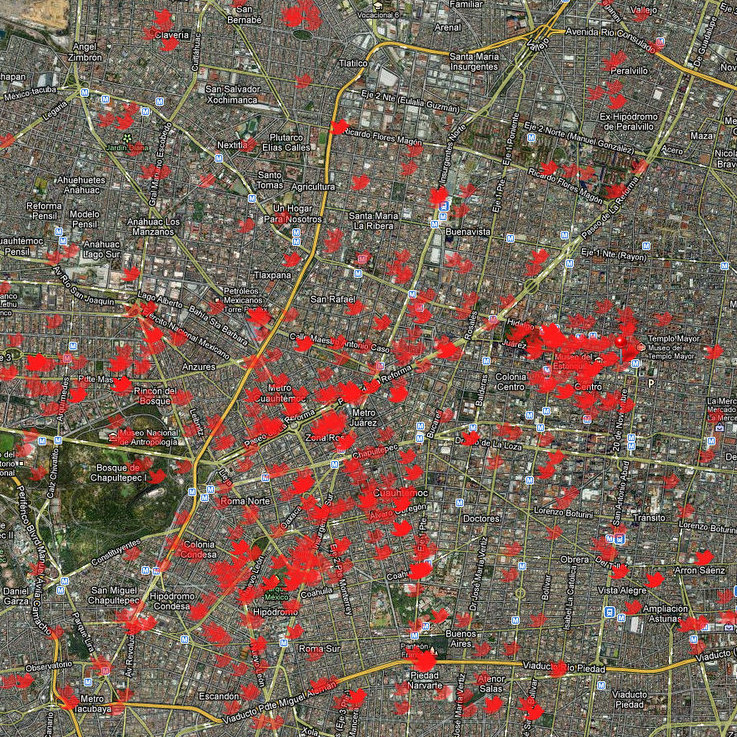
\includegraphics[width=\linewidth]{./maps/example2.jpg}
  \caption{Point pattern analysis}\label{fig:awesome_image2}
\endminipage\hfill
\minipage{0.32\textwidth}%
  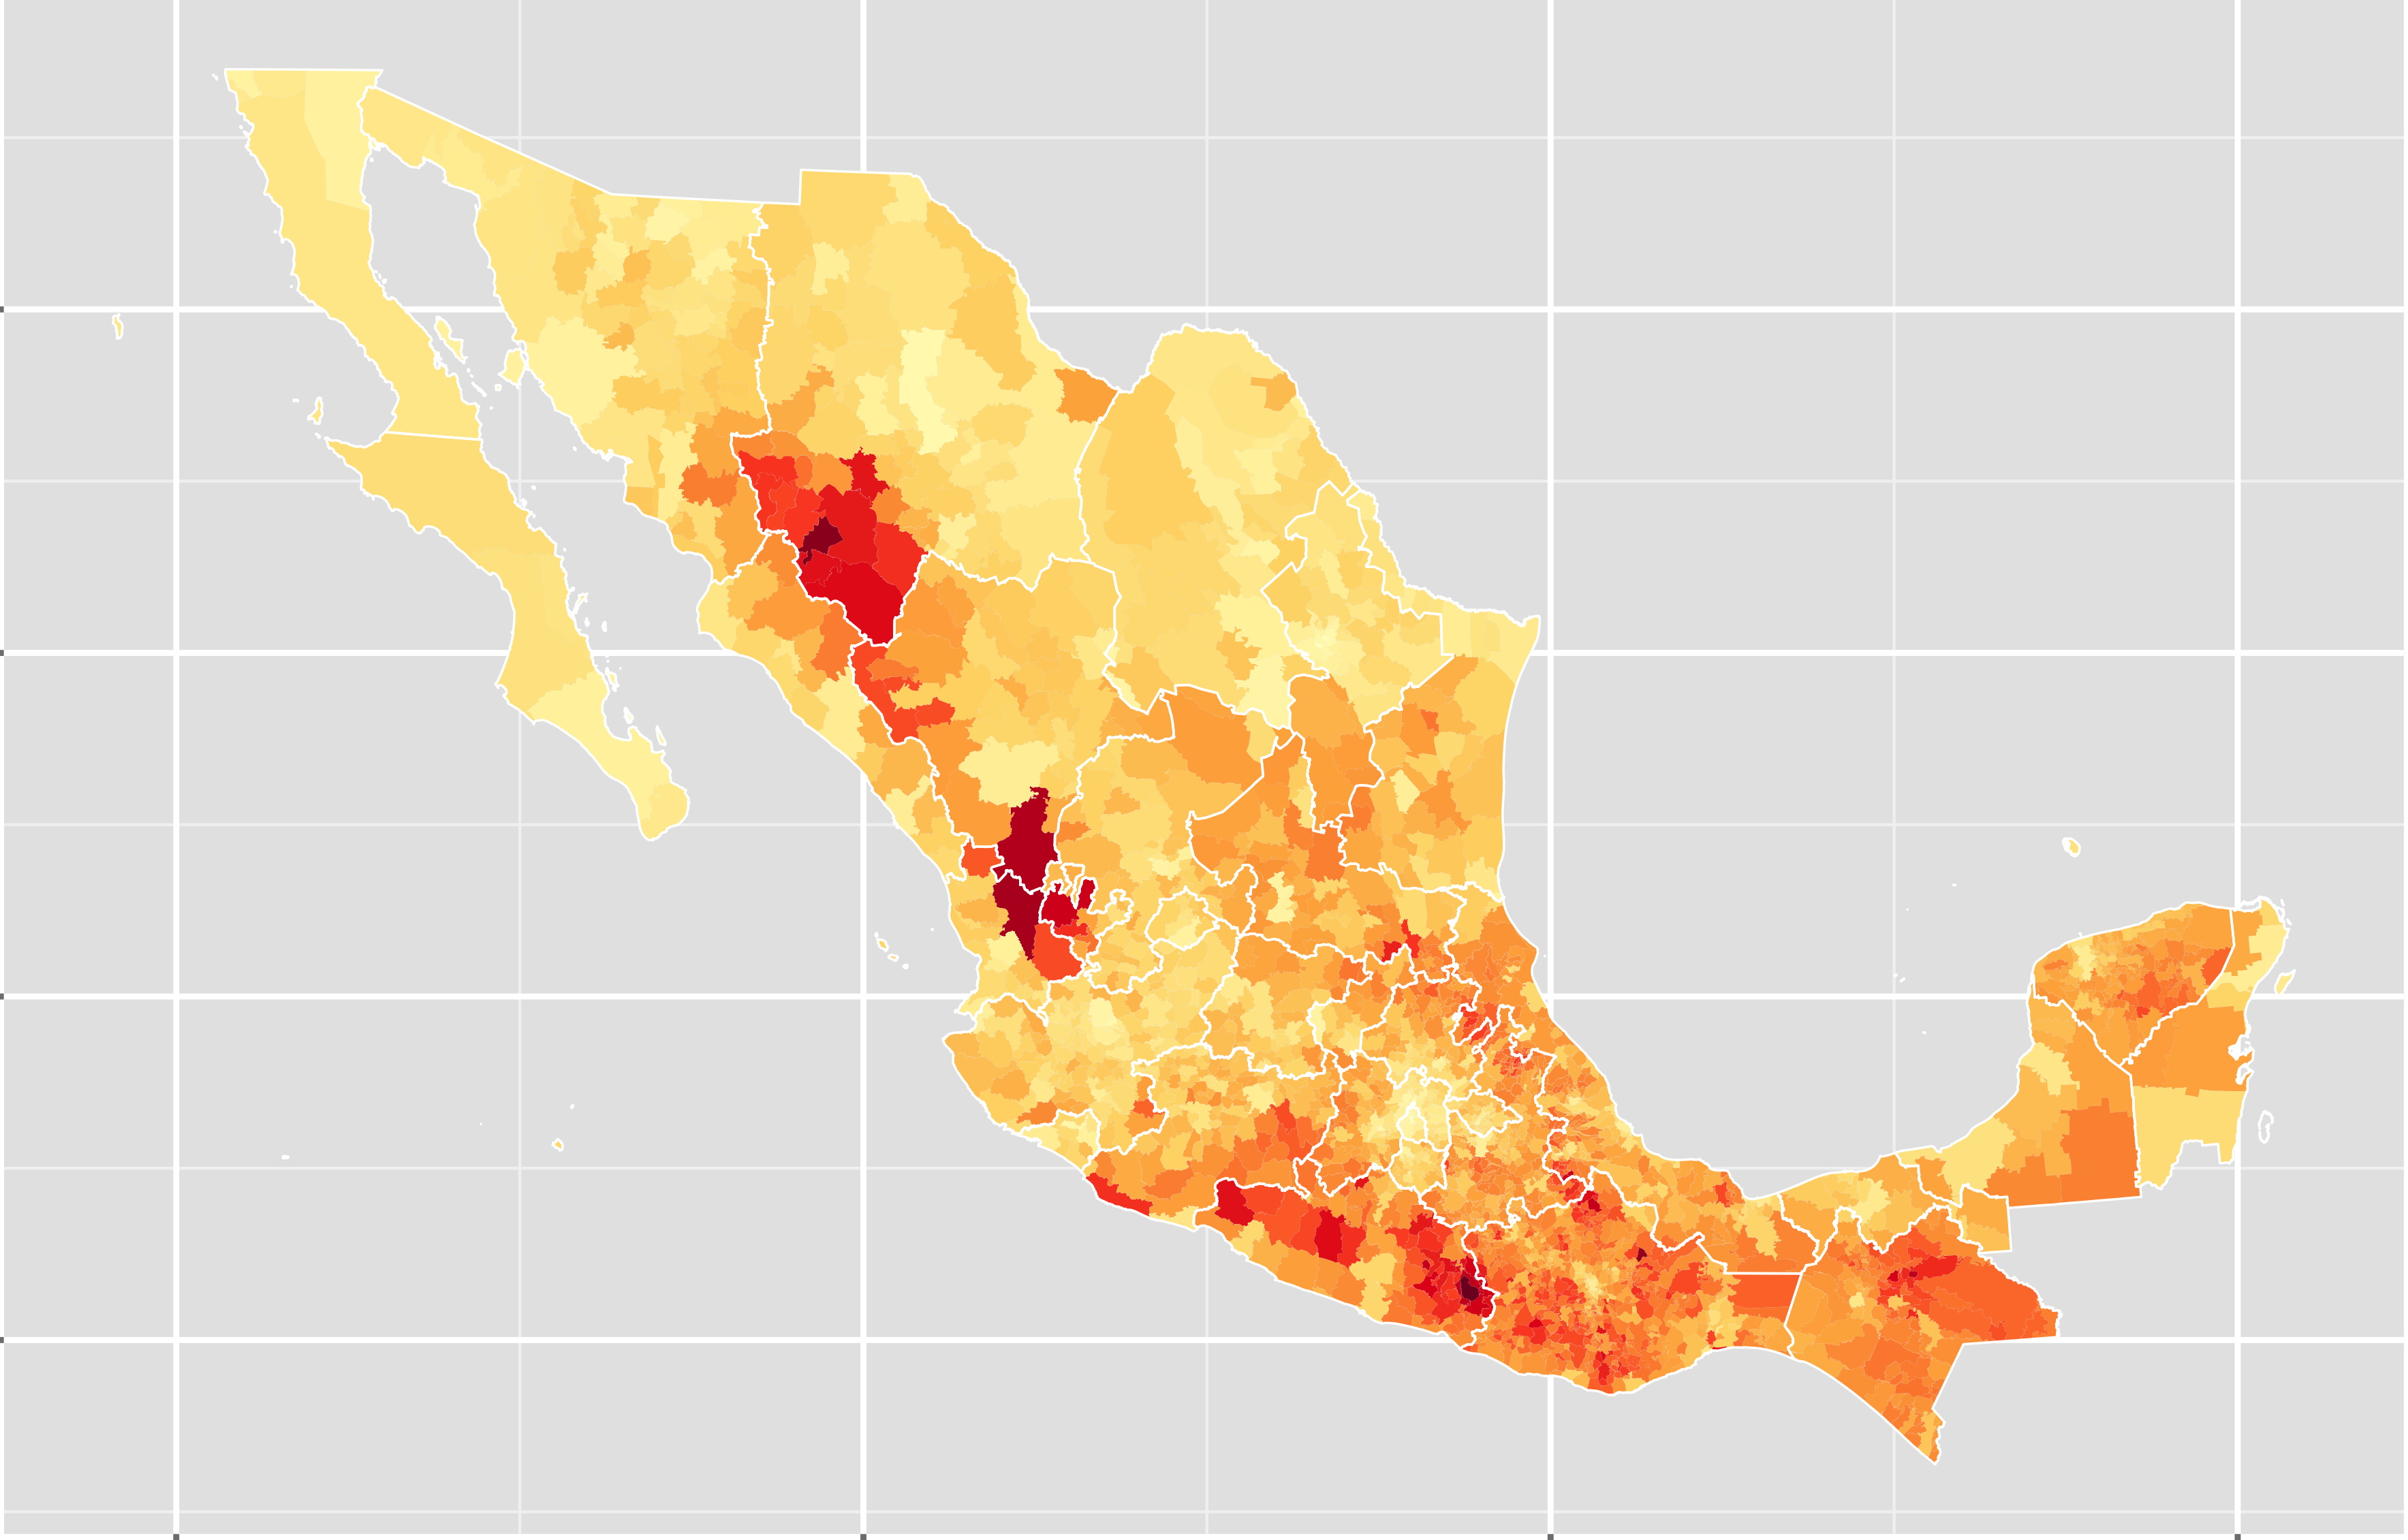
\includegraphics[width=\linewidth]{./maps/example3.png}
  \caption{Datos en retícula}\label{fig:awesome_image3}
\endminipage
\end{figure}
\end{frame}

\subsection{Autocorrelación Espacial}

\begin{frame}{Autocorrelación Espacial}
\begin{itemize}
\item Las observaciones realizadas en diferentes puntos espaciales pueden no ser independientes.
\item A esto se le llama autocorrelación espacial, la cual mide el grado en el que un fenómeno de interés se relaciona consigo mismo en el espacio.
\item Las pruebas de autocorrelación espacial examinan si el valor observado de una variable en algún lugar es independiente de los valores de la misma variable en lugares cercanos o contiguos.
\end{itemize}
\end{frame}

\begin{frame}
\begin{itemize}
\item \textbf{Autocorrelación espacial positiva} indica que los valores similares están cercanos entre sí, o aglomerados, en el espacio.
\item \textbf{Autocorrelación espacial negativa} indica que valores vecinos no son similares, o equivalentemente, que valores similares están dispersos en el espacio.
\item \textbf{Autocorrelación espacial nula} indica que el patrón espacial es aleatorio.
\end{itemize}
\end{frame}

\begin{frame}{Matriz de pesos}
  Debemos definir primero qué significa que dos observaciones sean cercanas a través de una matriz de pesos $W$.
  \begin{itemize}
  \item  \textbf{Contigüidad binaria:}
    \begin{equation} \label{binw}
      w_{ij}=  \begin{cases} 1 & \mbox{si la región } i \mbox{ comparte frontera con } j \\ 
      0 & \mbox{e.o.c.} 
      \end{cases}
    \end{equation}
  \item \textbf{Distancia:} Distancia entre dos puntos o regiones.
  \item \textbf{Frontera en común:} Longitud de la frontera entre dos regiones.
  \item \textbf{Combinación de frontera y distancia}
  \end{itemize}

  Podemos ajustar $W$ de tal forma que la suma de los pesos por renglón sea igual a $1$  utilizando una matriz estandarizada por filas.
\end{frame}

% \begin{frame}
% Podemos ajustar $W$ de tal forma que la suma de los pesos por renglón sea igual a $1$  utilizando una matriz estandarizada por filas donde dividimos cada elemento $w_{ij}$ por la suma de los pesos de los vecinos de la región $i$ obteniendo una matriz $W_{std}$ donde

% \begin{equation}
% w_{std,ij}=\dfrac{w_{ij}}{\displaystyle \sum_{j=1}^n w_{ij}}.
% \end{equation}
% \end{frame}

\begin{frame}{Pruebas de Autocorrelación Espacial}
  \begin{itemize}
    \item Consideremos un área de estudio particionada en $n$ regiones. 
    \item Sea $Y$la variable de estudio, $y_i$ es la observación de la variable $Y$ en la región $i$.
    \item Si $Y$ es de escala continua u ordinal, utilizamos los coeficientes $\mathcal{I}$ de Moran y $\mathcal{C}$ de Geary.
    \item Si $Y$ es nominal, utilizamos el estadístico de conteo de fronteras (Join count).
  \end{itemize}
\end{frame}

\begin{frame}{Índice $\mathcal{I}$ de Moran}
Se basa en los productos cruzados de las desviaciones de la media y se calcula:

\begin{equation}
\mathcal{I} = \left( \dfrac{n}{ \sum_{i=1}^n \sum_{j=1}^n w_{ij}} \right) \left( \dfrac{\sum_{i=1}^n \sum_{j=1}^n w_{ij} (y_{i} - \bar{y}) (y_{j} - \bar{y}) }{ \sum_{i=1}^n (y_{i} - \bar{y})^2} \right).
\end{equation}
$\mathcal{I}$ no es como un coeficiente de correlación común, pues no pertenece necesariamente al intervalo $(-1,1)$. Usualmente $\mathcal{I} \in (-1,1)$
\end{frame}

\begin{frame}{Índice $\mathcal{C}$ de Geary}
Utiliza la suma de diferencias al cuadrado entre pares de observaciones como medida de variación. Está dado por

\begin{equation}
\mathcal{C} =  \left(\dfrac{n-1}{ 2 \sum_{i=1}^n \sum_{j=1}^n w_{ij}}\right)  \left( \dfrac{ \sum_{i=1}^n \sum_{j=1}^n w_{ij} (y_{i} - y_{j})^2}{ \sum_{i=1}^n (y_{i} - \bar{y})^2}\right).
\end{equation}

Toma valores en el intervalo $[0,2]$ donde 0 indica correlación espacial positiva perfecta y 2 indica correlación espacial negativa perfecta. 
\end{frame}

\begin{frame}{Distribución de $\mathcal{I}$ y $\mathcal{C}$}
  Bajo ciertas condiciones de regularidad, $\mathcal{I}$ y $\mathcal{C}$ se distribuyen normal a medida que $n$ aumenta. Los momentos de $\mathcal{I}$ y $\mathcal{C}$ pueden ser evaluados bajo alguna de los siguientes dos supuestos:
  \begin{enumerate}
    \item \textbf{Normalidad}: Asumimos que las observaciones $y_i$ son resultado de $n$ realizaciones de una población normal.
    \item \textbf{Aleatorización}: Consideramos el valor observado de $\mathcal{I}$ y $\mathcal{C}$ relativo al conjunto de todos los valores posibles que pueden tomar $\mathcal{I}$ y $\mathcal{C}$ si $y_1, y_2, ..., y_n$ fueran permutadas de manera aleatoria repetidamente alrededor de las regiones dentro del área de estudio.
  \end{enumerate}
\end{frame}

\begin{frame}{Momentos de $\mathcal{I}$ y  $\mathcal{C}$}
  Coeficiente $\mathcal{I}$
  \begin{eqnarray}
  \E\left[\mathcal{I} \right] = -\dfrac{1}{n-1}, &
  \E\left[\mathcal{I}^2\right] =  \dfrac{n^2S_1-nS_2+3S_0^2}{S_0^2(n^2-1)}
  \end{eqnarray}

  Coeficiente $\mathcal{C}$
  \begin{eqnarray}
  \E\left[\mathcal{C}\right] = 1, & 
  \Var(\mathcal{C}) =\dfrac{(2S_1+S_2)(n-1)-4S_0^2}{2(n+1)S_0^2}
  \end{eqnarray}

  Donde 
  \begin{align}
    S_0 = \sum_{i=1}^n \sum_{j=1}^n w_{ij}, && S_1 = \dfrac{1}{2} \sum_{i=1}^n \sum_{j=1}^n  \left( w_{ij}+w_{ji} \right)^2, & S_2 = \sum_{i=1}^n  \left( w_{i.}+w_{.i} \right)^2. \nonumber
  \end{align}

  \begin{eqnarray}
  w_{i.} = \sum_{j=1}^n w_{ij} & \mbox{ y } & w_{.j} = \sum_{i=1}^n w_{ij}.\nonumber
  \end{eqnarray}
\end{frame}

\begin{frame}{Variables Discretas: Estadístico join-count}
  \begin{itemize}
  \item Se utiliza si $Y$ es categórica.
  \item Supongamos que $Y$ cuenta con 2 clases $y_{i}\in \lbrace 0,1 \rbrace$. Mapeando $y$ en 2 colores , W si $y_{i}=0$ y B si $y_{i}=1$ cada frontera o unión entre dos regiones es clasificada como $WW$ (0-0), $BB$ (1-1) ó $BW$ (1-0).
  \item Si el número de uniones $BB$ es significativamente mayor del esperado por sorteo, habrá autocorrelación espacial positiva;  si es significativamente menor, autocorrelación espacial negativa; y si es aproximadamente el mismo, autocorrelación espacial nula.
  \end{itemize}
\end{frame}

\begin{frame}{Distribución de los conteos}
  \begin{itemize}
    \item $BB$, $BW$ y $WW$ asintóticamente se distribuyen normal.
    \item Los parámetros $\mu$ y $\sigma^2$ de los coeficientes pueden ser evaluados bajo uno de las dos supuestos:
    \begin{enumerate}
      \item \textbf{Muestreo con reemplazo}: cada una de las regiones es etiquetada como $B$ o $W$ independientemente con probabilidad $p_B$ y $p_W=1-p_B$ respectivamente. 

      \item \textbf{Muestreo sin reemplazo}: cada región tiene la misma probabilidad, a priori, de ser $B$ o $W$, pero la codificación está sujeta a la restricción de que hay $n_B$ regiones con color $B$ y $n_W$ regiones con color $W$, y $n_a+n_b=n$.
    \end{enumerate}
  \end{itemize}
\end{frame}

\begin{frame}{Generalización a $k > 2$}
Generalmente contamos con más de dos clases ($k > 2$), tenemos que cada una de las $n$ regiones pertenece a alguna de las $k$ categorías. Así, $n_{1}$ regiones son de tipo 1, $n_{2}$ regiones son de tipo 2 y así sucesivamente, y $n_{k}$ regiones son de tipo $k$. De tal manera:
\begin{equation}
n_{1}+n_{2}+...+n_{k}=n. \nonumber
\end{equation}

Definimos $N_{rr}$ como el número de uniones entre regiones del tipo $rr$,  $N_{rs}$ el número de uniones del tipo $rs$, con  $r,s \in \{1,2, \dots, k\}$.
\end{frame}

\begin{frame}{Momentos de los estadísticos $N_{rr}$ bajo muestreo sin reemplazo}
  \begin{equation}
  \mu = \dfrac{S_0n_r(n_r-1)}{2n(n-1)} ,
  \end{equation}

  \begin{equation}
  \sigma^2 = \dfrac{S_1n_r^{(2)}}{4n^{(2)}} + \dfrac{(S_2-2S_1)n_r^{(3)}}{4n^{(3)}} + \dfrac{(S_0^2+S_1-S_2)n_r^{(4)}}{4n^{(4)}}-\mu^2 .
  \end{equation}
  donde 
    $n^{(k)}=n(n-1)(n-2)\dots(n-k+1)$.


\end{frame}

\begin{frame}{Pruebas de hipótesis}
  \begin{itemize}
    \item La hipótesis nula $H_0$ es de no autocorrelación espacial,
    \item Hay dos procedimientos a seguir:
    \begin{enumerate}
      \item Utilizando el supuesto de normalidad.
      \item Si dudamos del supuesto de normalidad, podemos utilizar simulaciones de Monte Carlo.
      Es recomendable hacer esta prueba ya que la función de densidad del estadístico es sensible a los siguientes factores:
      \begin{itemize}
        \item La forma de las regiones en el área de estudio.
        \item Los pesos $w_{ij}$ utilizados.
        \item La distribución de la variable $Y$.
        \item El tamaño de la muestra $n$.
      \end{itemize} 
    \end{enumerate}
  \end{itemize}
\end{frame}

\begin{frame}{Simulaciones de Monte Carlo}
    \begin{enumerate}
    \item Permutamos aleatoriamente las etiquetas $y_1, y_2, \dots, y_n$ a través de las regiones. 
    \item Calculamos el estadístico de interés, digamos $\mathcal{I}$, con las etiquetas permutadas. 
    % Si la variable $Y$ es continua hay $n!$ permutaciones posibles; si es discreta, $\dbinom{n}{n_1 n_2 \dots n_k}$.
    \item Repetimos 1. y 2. $n_{sim}$ veces, obteniendo una muestra de tamaño $n_{sim}$ de $\mathcal{I}$. 
    \item Comparamos el valor observado del estadístico con la muestra obtenida. 
    \end{enumerate}
\end{frame}

\section{Resultados}
\subsection{Análisis Exploratorio}
\begin{frame}{Base de Datos}
  \begin{itemize}
  \item Base de datos:``Índice de Marginación por Entidad Federativa y Municipio 2010''. 
  \item $2,456$ municipios y cada una tiene $12$ atributos.
  \item 9 de estos atributos son indicadores de marginación. 
  \item Los atributos restantes son el índice de marginación, índice de marginación escalado de 0 a 100 y grado de marginación. 
  \item El índice de marginación es un resumen de estos atributos y el grado de marginación es una categorización de éste.
  \end{itemize}
\end{frame}

\begin{frame}{Análisis Exploratorio: Índice de Marginación}
  \begin{figure}[!ht]
  \centering
  % 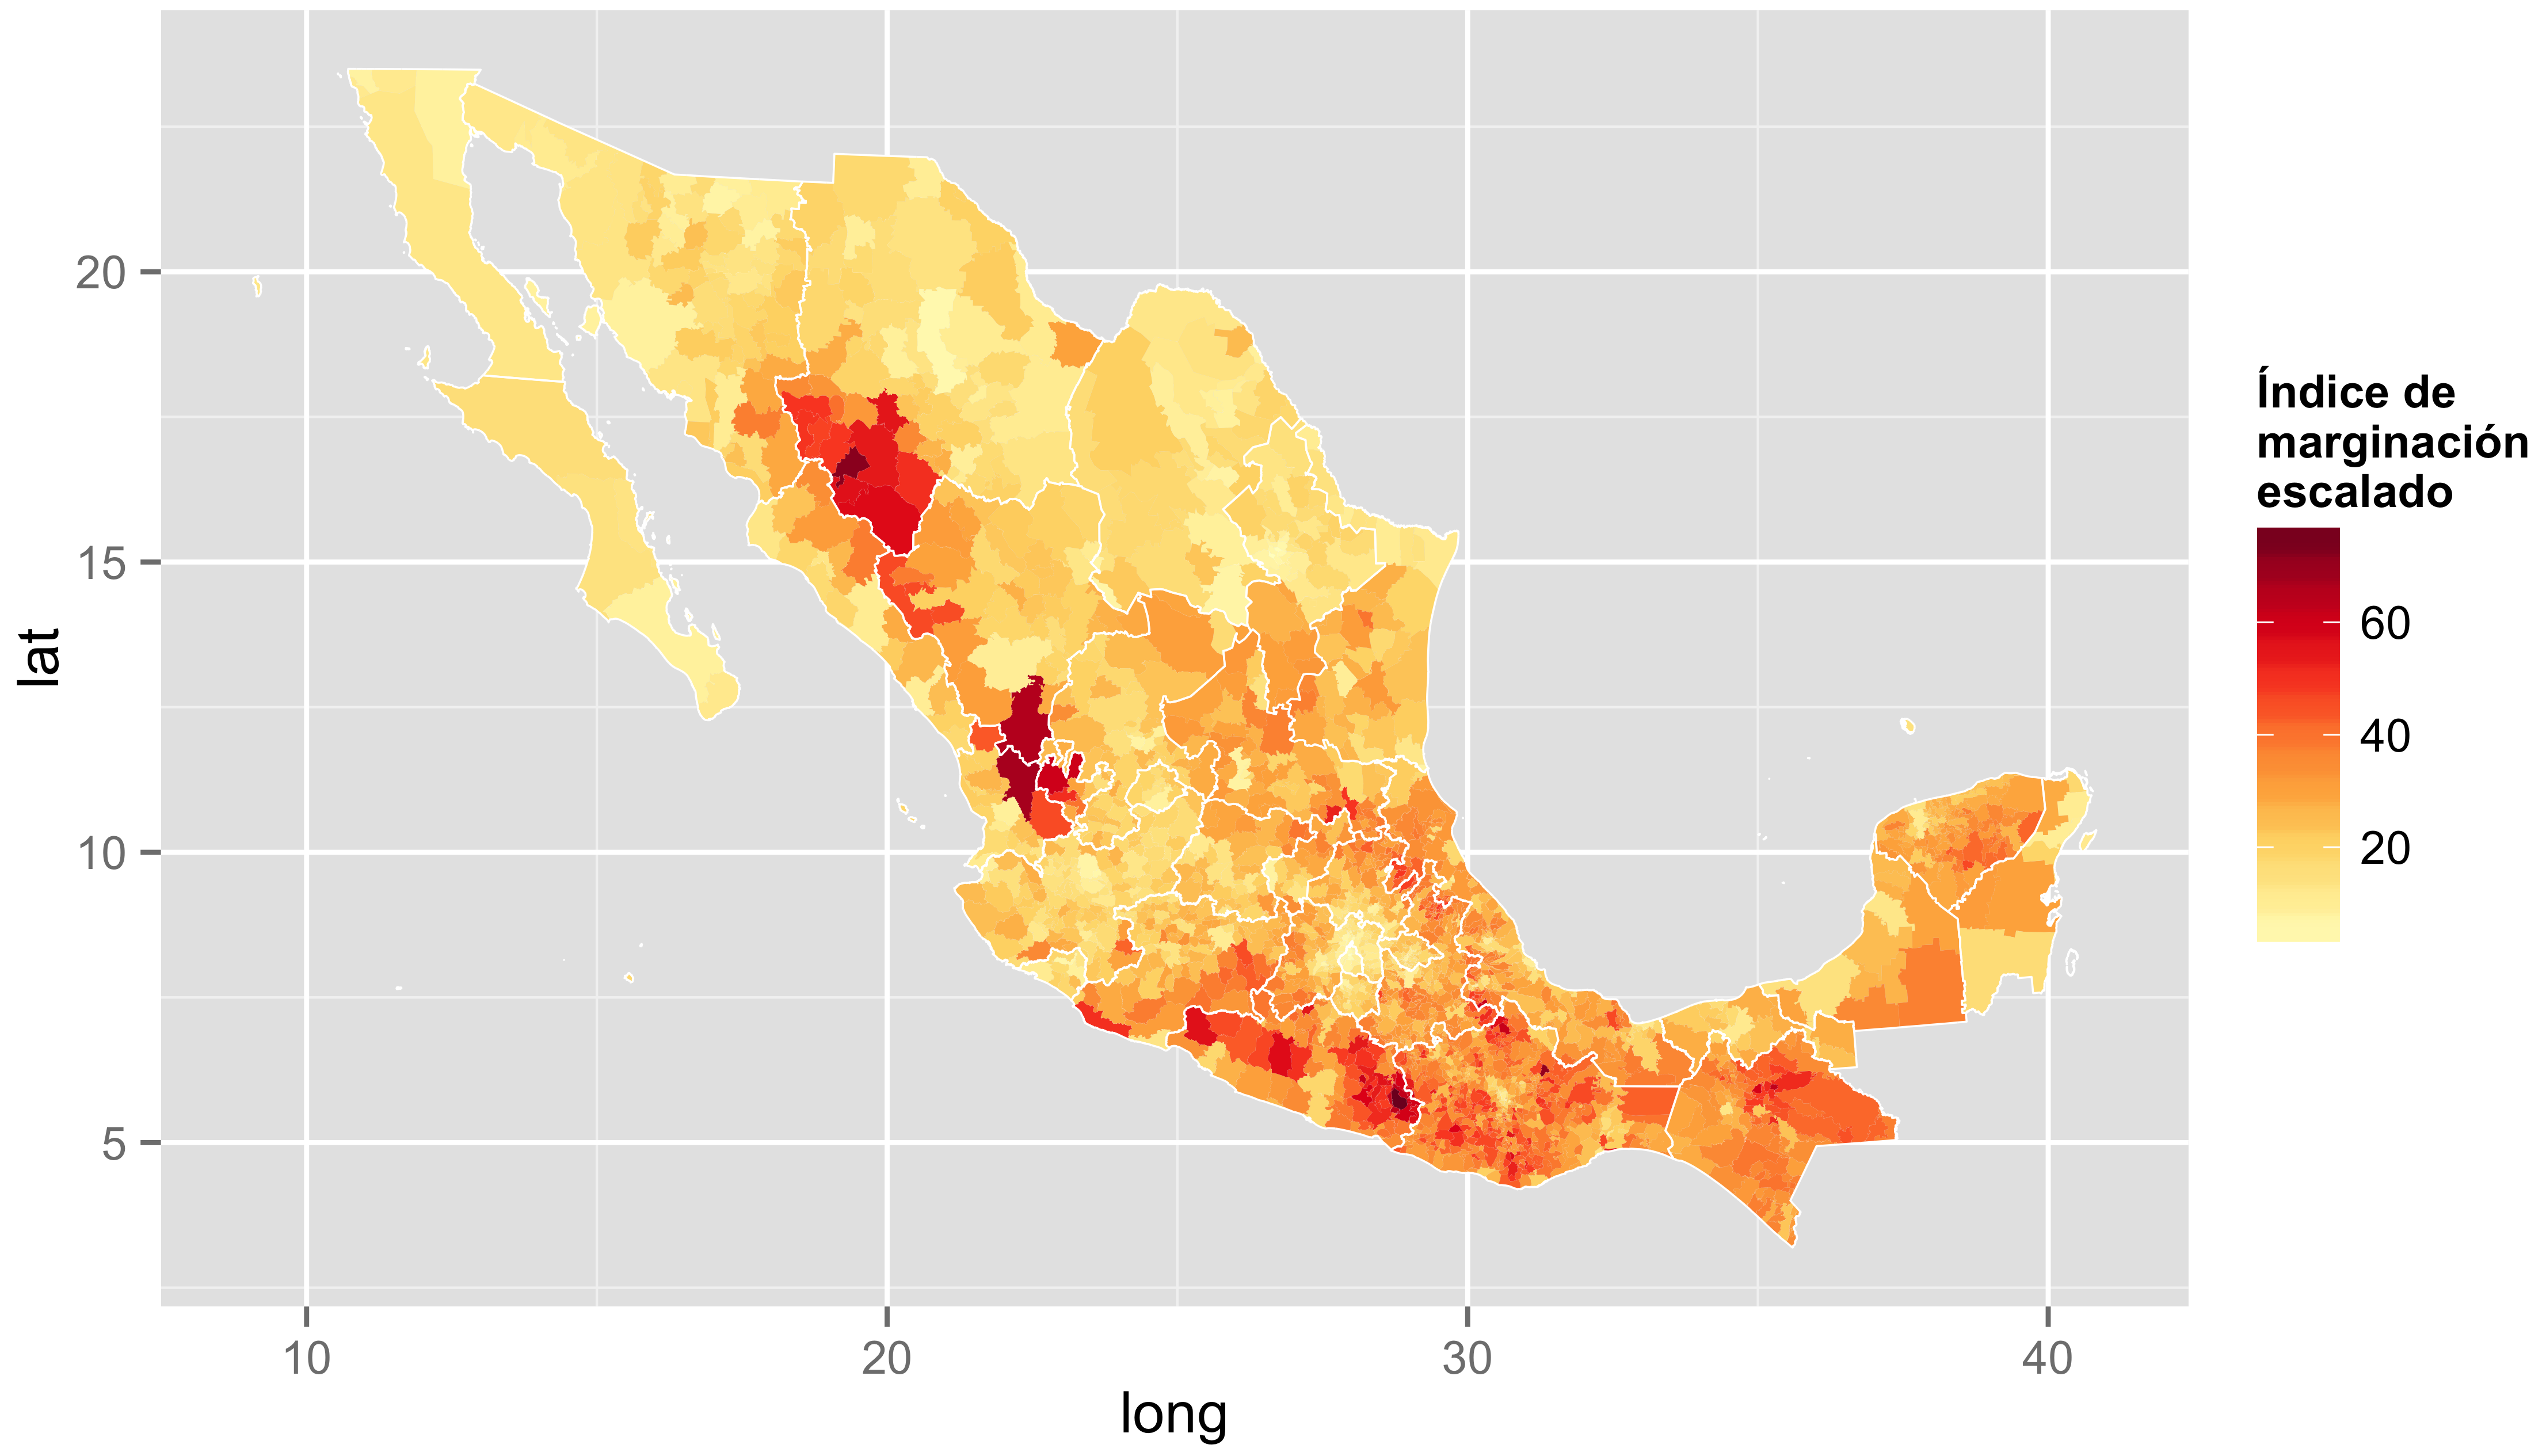
\includegraphics[scale=.20]{./maps/mapmarg.png} \\
  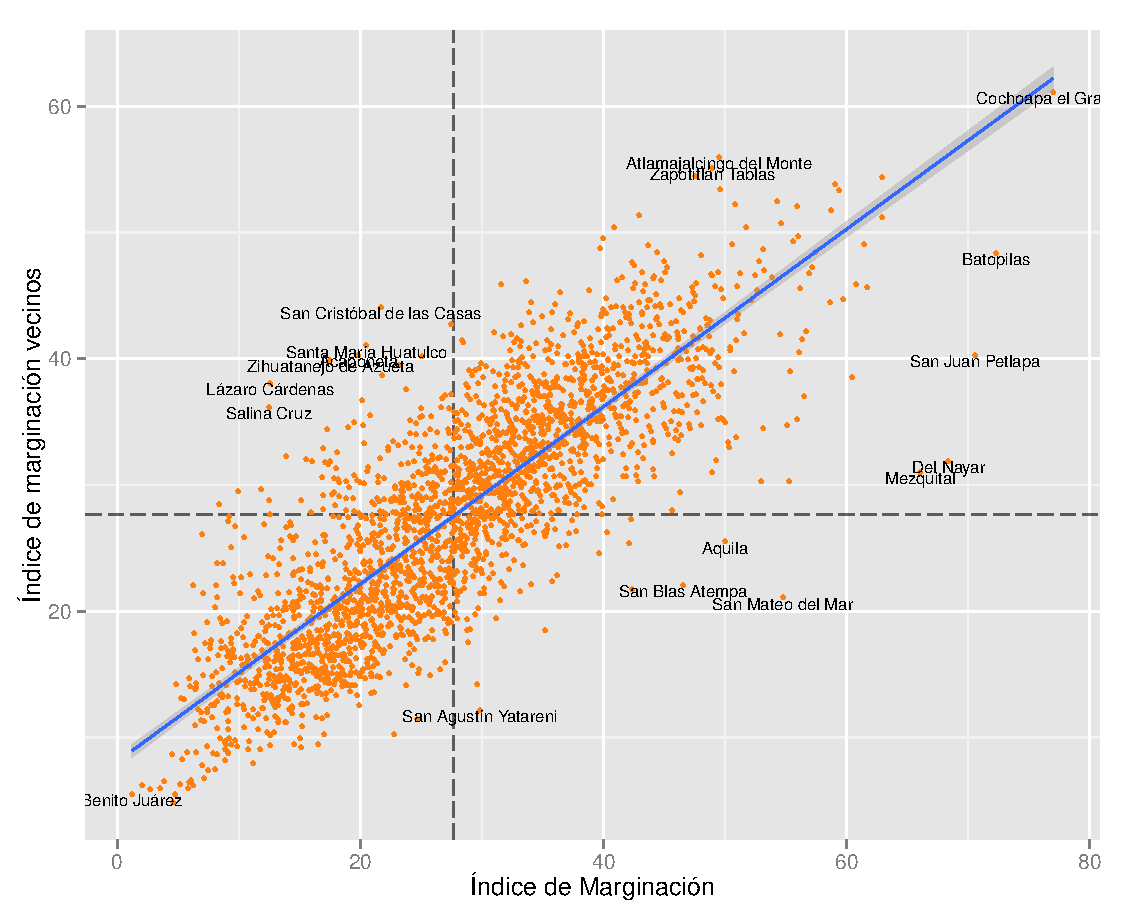
\includegraphics[width=.8\textwidth]{./plots/moran_plot.pdf} \\
  % \caption{Gráfica de Moran para índice de marginación.}
 
  \end{figure}
\end{frame}

\begin{frame}
  \begin{figure}[!ht]
  \centering
  % 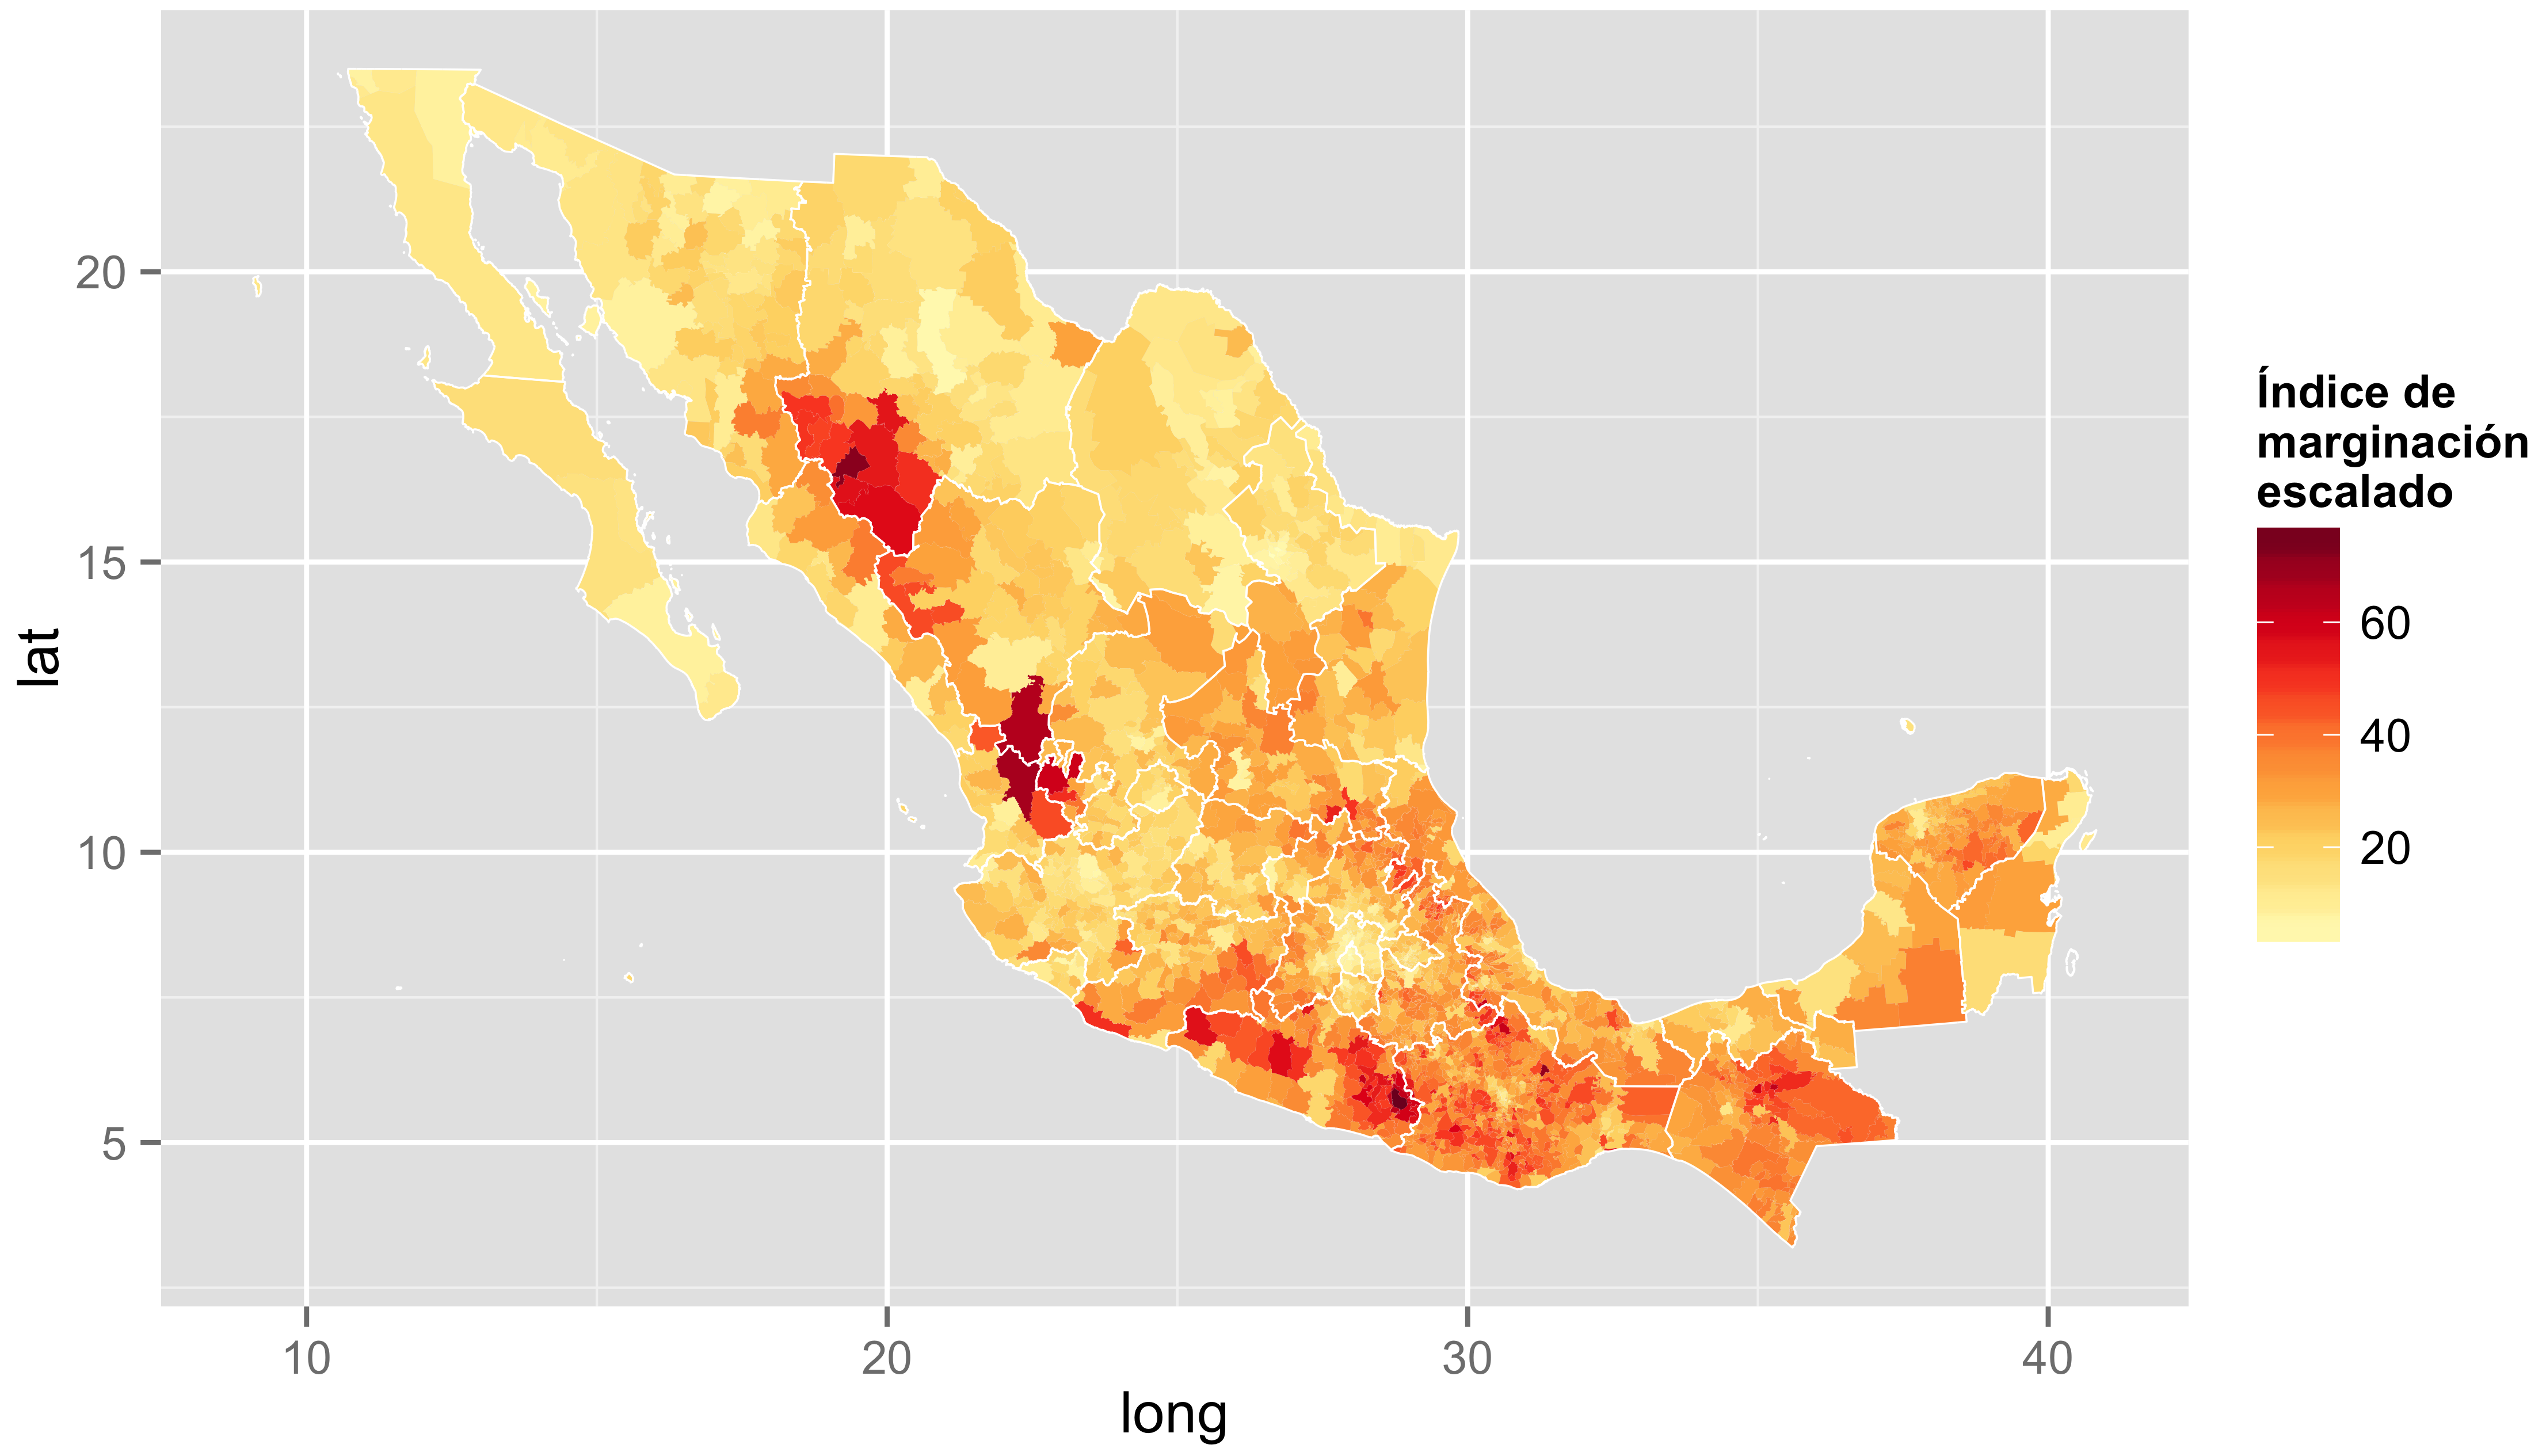
\includegraphics[scale=.20]{./maps/mapmarg.png} \\
  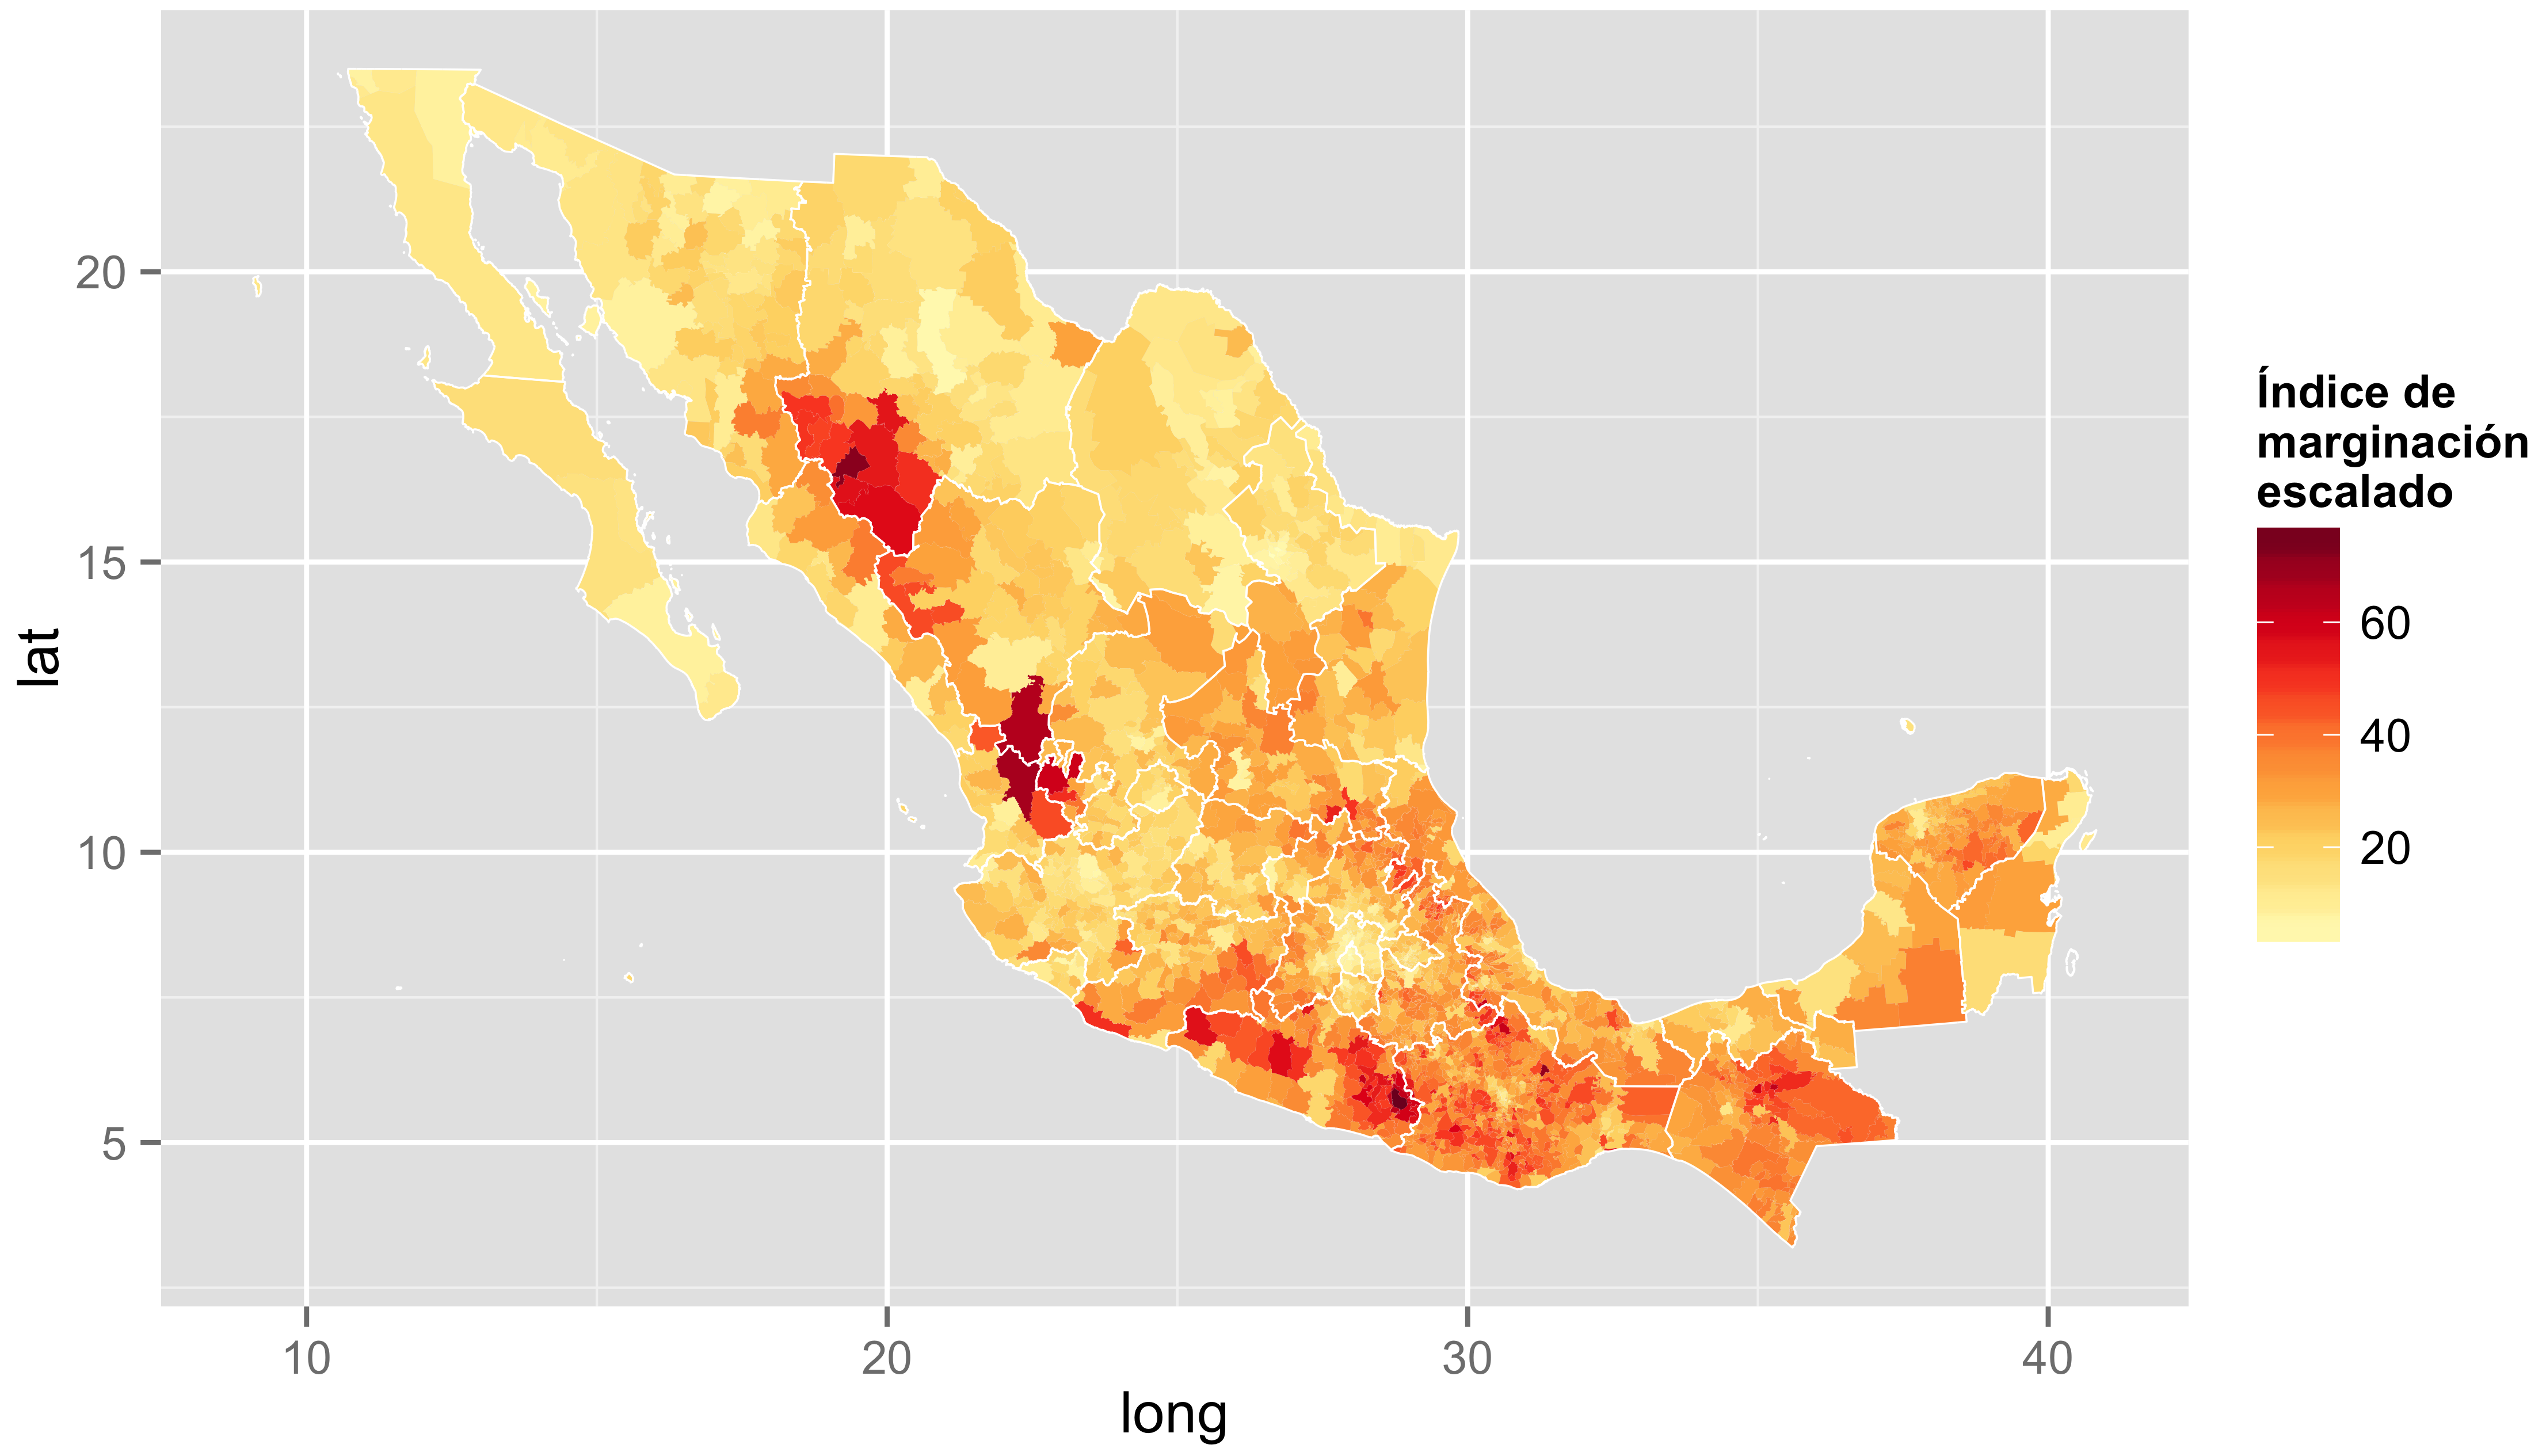
\includegraphics[width=1\textwidth]{./maps/mapmarg.png} \\
  \end{figure}
\end{frame}
\subsection{Pruebas de Autocorrelación Espacial para el índice de marginación}
\begin{frame}{Pruebas de Autocorrelación Espacial para el índice de marginación}
\begin{itemize}
\item Se escogen pesos binarios estandarizados.
\item Hipótesis alternativa, autocorrelación espacial positiva
\item Obtenemos: 
$\Hat{\mathcal{I}} = 0.703$ y $\Hat{\mathcal{C}} = 0.2943260693$
\item Bajo el supuesto de normalidad: $z(\mathcal{I}) = 57.6933$ y $z(\mathcal{C}) = 51.0396$
\item Utilizando simulaciones de Monte Carlo con $n_{sim}=9999$:

\begin{figure}[!ht]
\minipage{0.4\textwidth}
  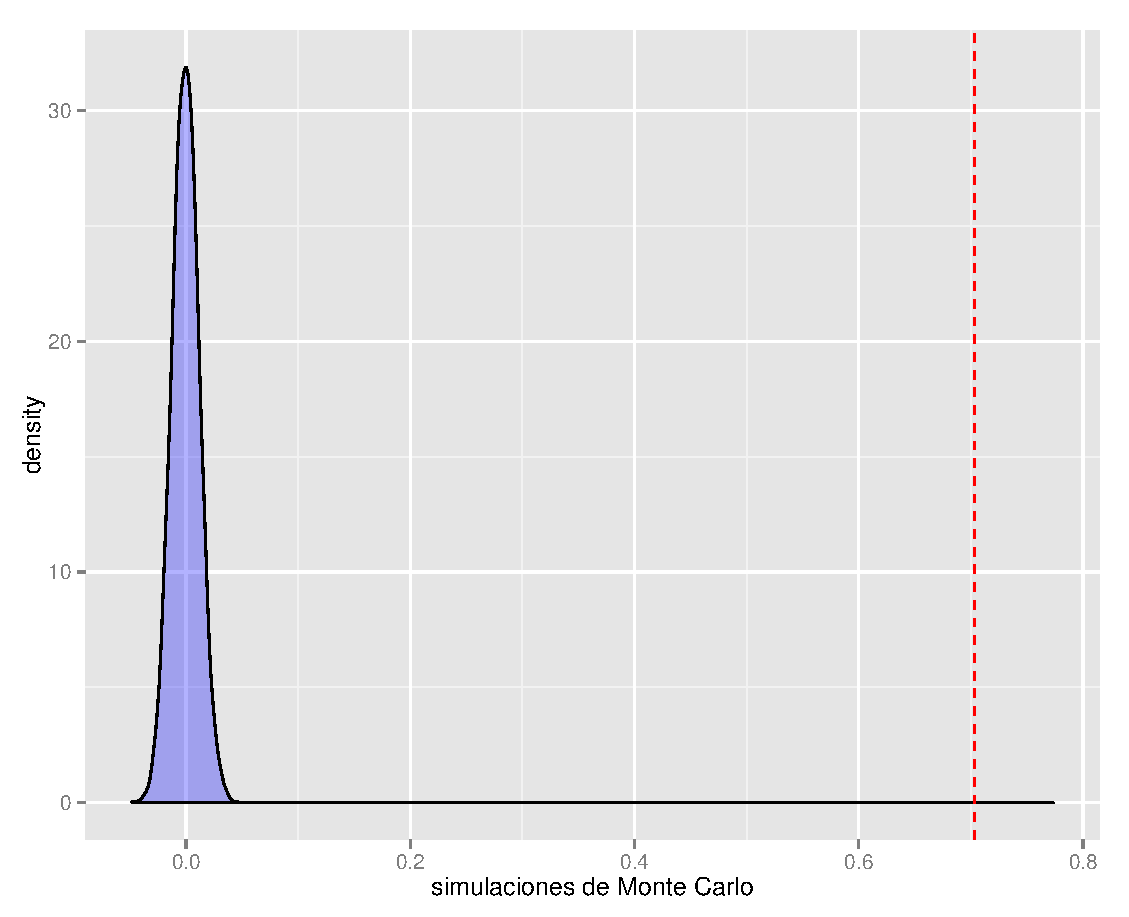
\includegraphics[width=\linewidth]{./plots/moran_density.pdf}
  \caption{Simulaciones de $\mathcal{I}$}
\endminipage\hfill
\minipage{0.4\textwidth}
  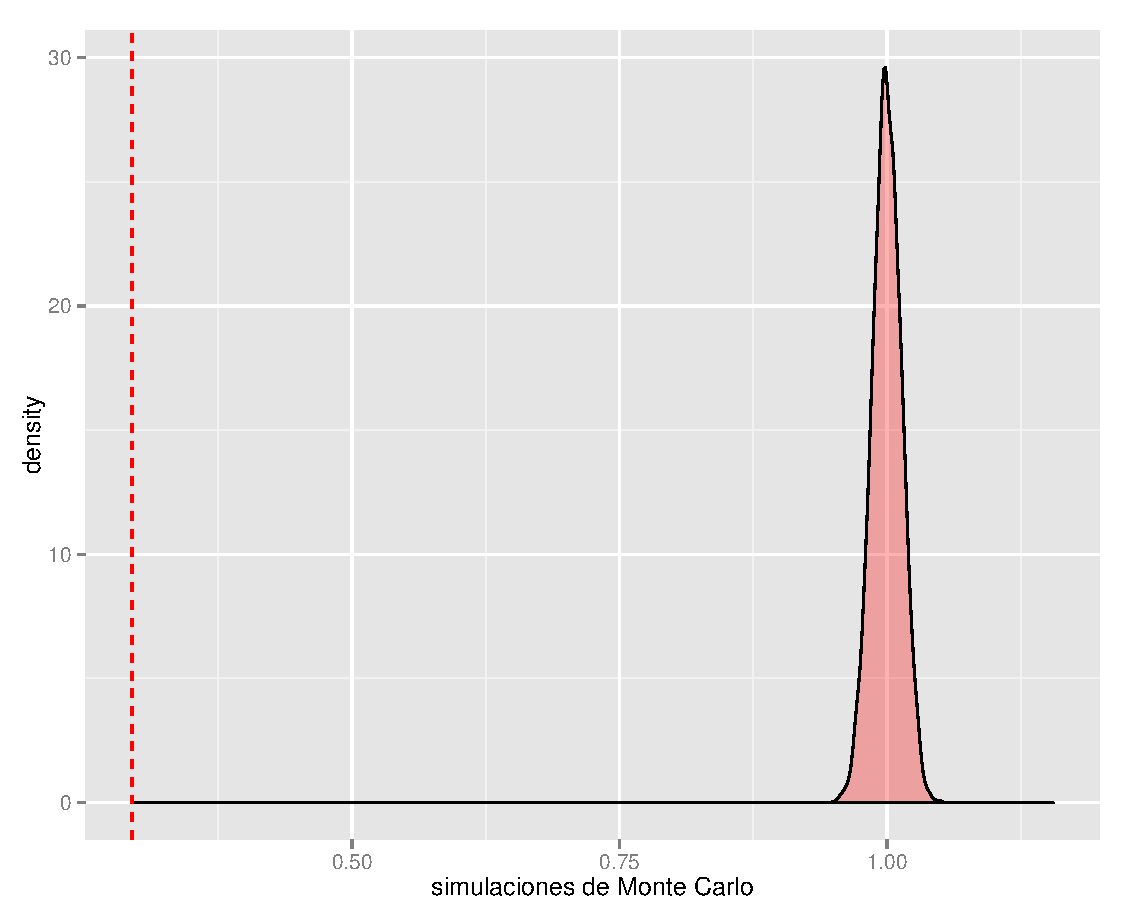
\includegraphics[width=\linewidth]{./plots/geary_density.pdf}
  \caption{Simulaciones de $\mathcal{C}$}
\endminipage\hfill
\end{figure}

\end{itemize}
\end{frame}

% \begin{frame}
% \Huge{Hay autocorrelación espacial positiva para el índice de marginación!}
% \end{frame}

\subsection{Análisis de Conglomerados esférico}
\begin{frame}{K-medias esféricas: escoger $K^*$}
  \begin{itemize}
  \item Escogemos $K^*$ utilizando el estadístico Gap.
  \item Utilizando $M=10$ y $B=100$:
  \begin{figure}[!htb]
    \centering
    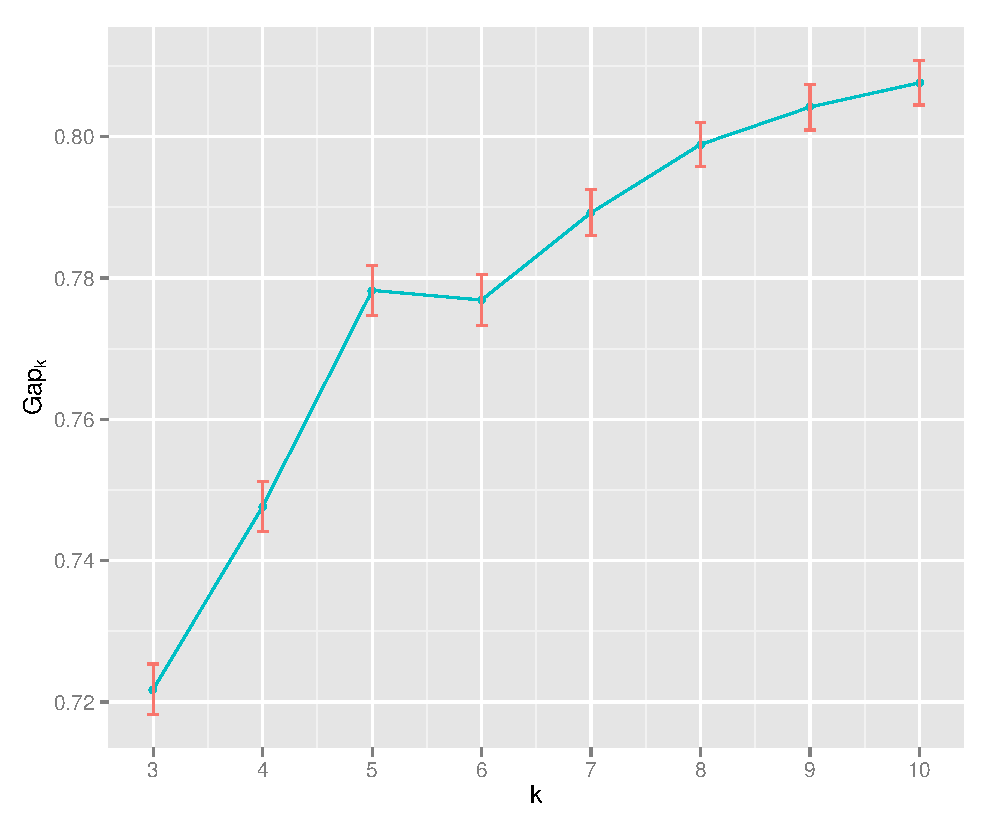
\includegraphics[width=.6\textwidth]{./plots/gap_plot.pdf}
  \end{figure}
  \item Obtenemos $K^*=5$
  \end{itemize}
\end{frame}

\begin{frame}{Reultados K-medias esféricas}
  \begin{enumerate}
  \item En el primer grupo cayeron municipios con localidades de pocos habitantes y con grado marginación de media a bajo. 
  \item En el segundo, cayeron los municipios más marginados cuyo principal rasgo es la carencia de agua entubada.
  \item El tercer grupo tiene municipios con grado de marginación de medio a alto, lo que lo separa del grupo dos es que tiene mayor porcentaje de viviendas con agua entubada.
  \item En el cuarto, se agruparon los municipios con menor grado de marginación.
  \item En el quinto, cayeron municipios con características similares al del primer grupo pero se diferencía en que cuenta con localidades más grandes.
  \end{enumerate}
\end{frame}

\begin{frame}{Distribución de los grupos}
  \begin{figure}[!ht]
    \centering
    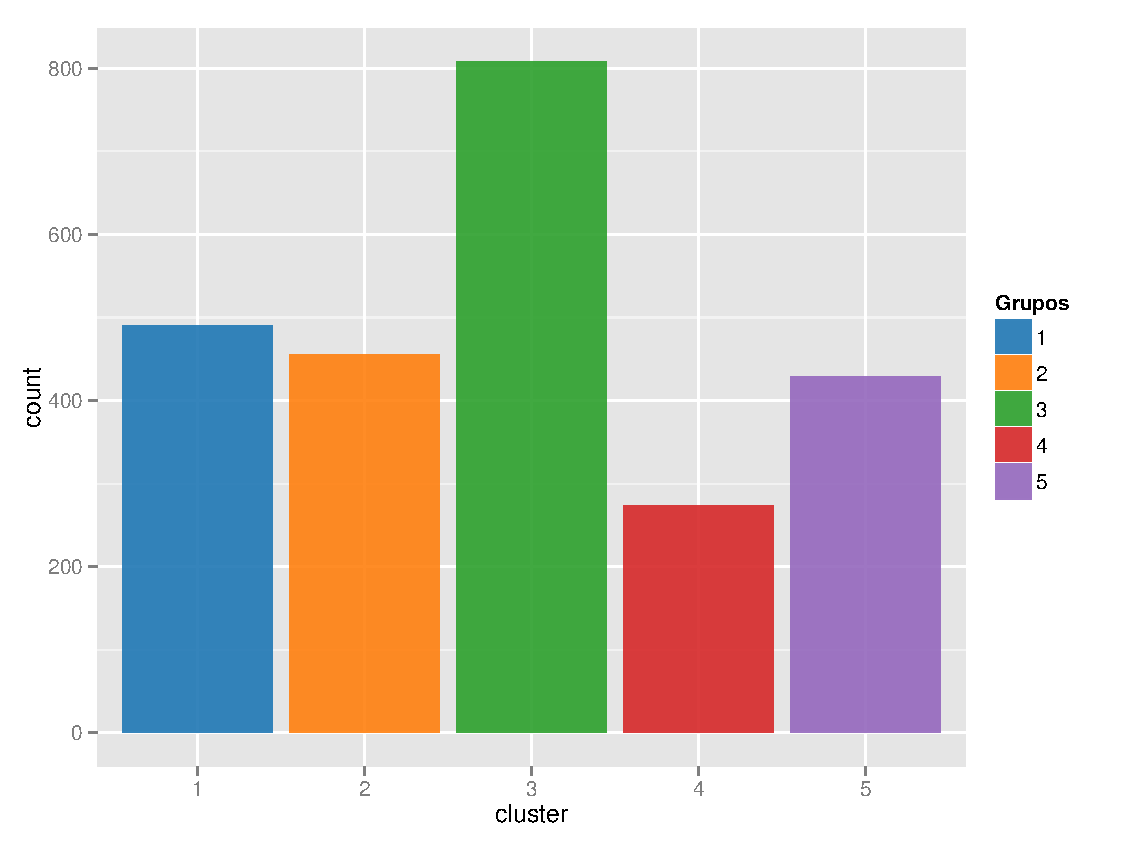
\includegraphics[width=.4\textwidth]{./plots/clustering_plot.pdf}
  \end{figure}
  \begin{table}[!ht]
  \centering
  \begin{tabular}{rrr}
    \hline
      & conteo & \% \\ 
    \hline
    1 & 490 & 20\% \\ 
    2 & 455 & 19\% \\ 
    3 & 808 & 33\% \\ 
    4 & 274 & 11\% \\ 
    5 & 429 & 17\% \\ 
     \hline
  \end{tabular}
  \end{table}
\end{frame}
\begin{frame}{Municipios coloreados por grupo}
  \begin{figure}[!ht]
    
    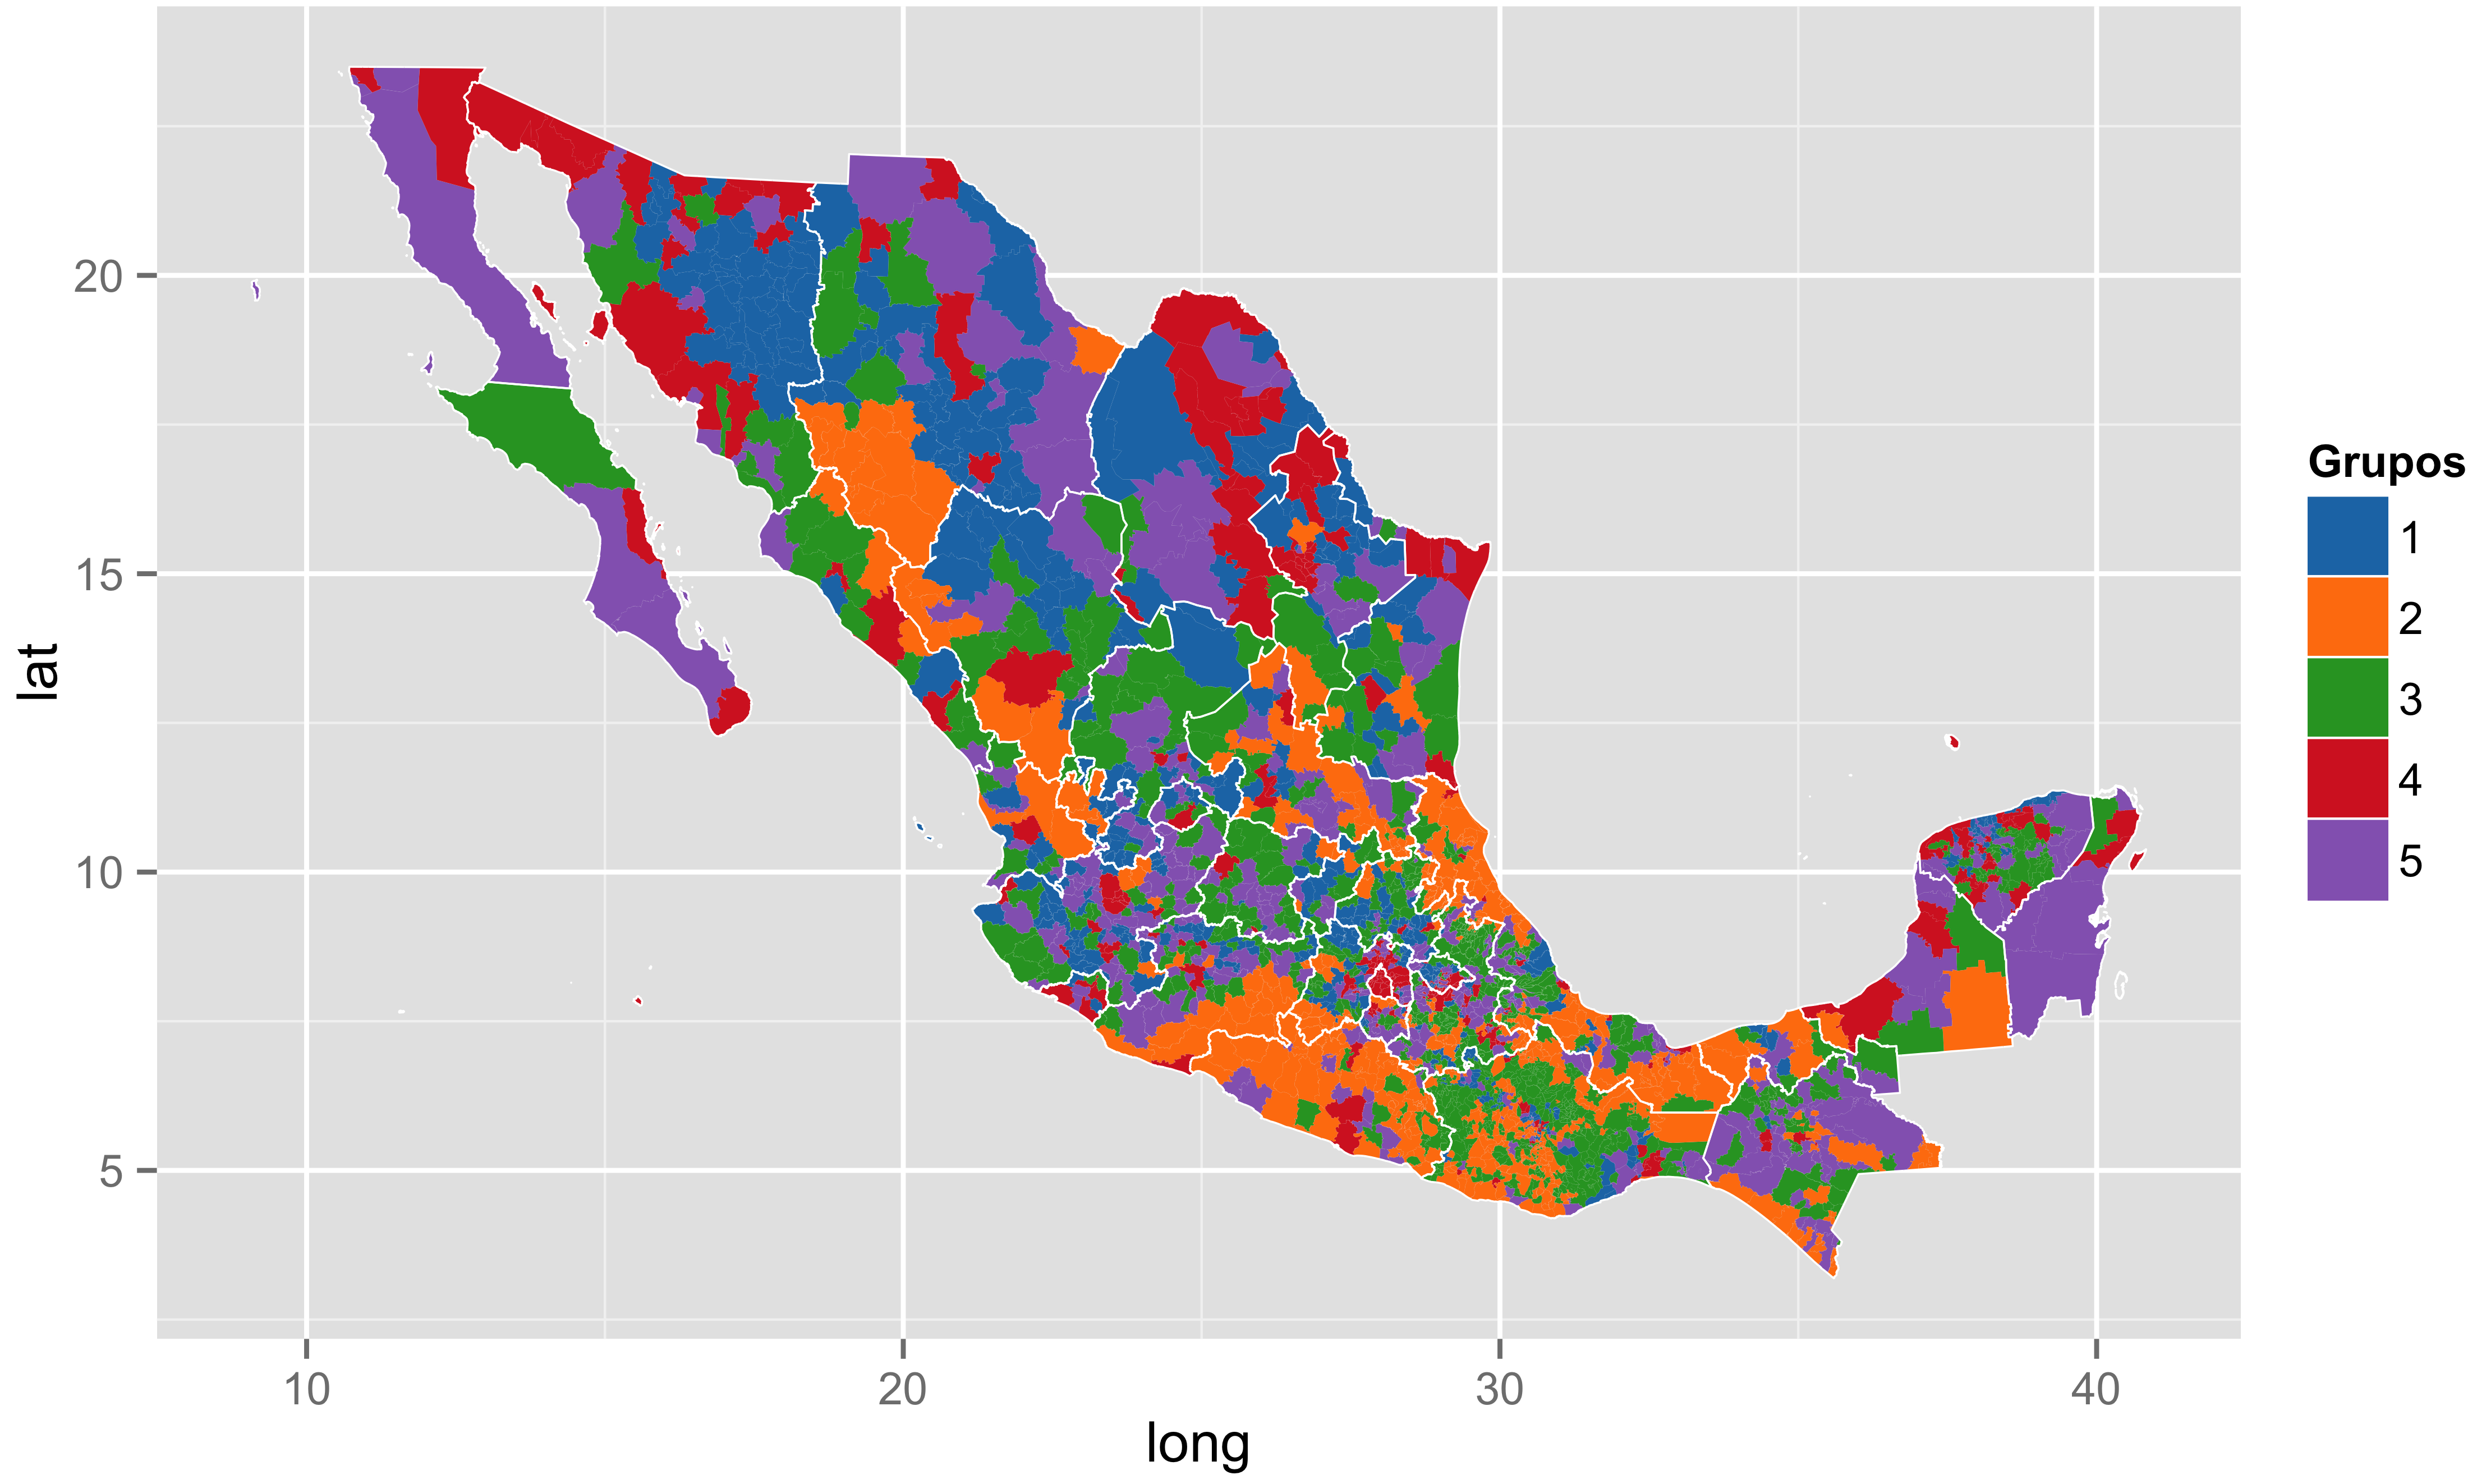
\includegraphics[width=1\textwidth]{./maps/map5g.png}
  \end{figure}
\end{frame}

\subsection{Pruebas de Autocorrelación Espacial para los clusters}
\begin{frame}{¿Existe autocorrelación espacial positiva?}
  \begin{figure}[!ht]
  \minipage{0.5\textwidth}
    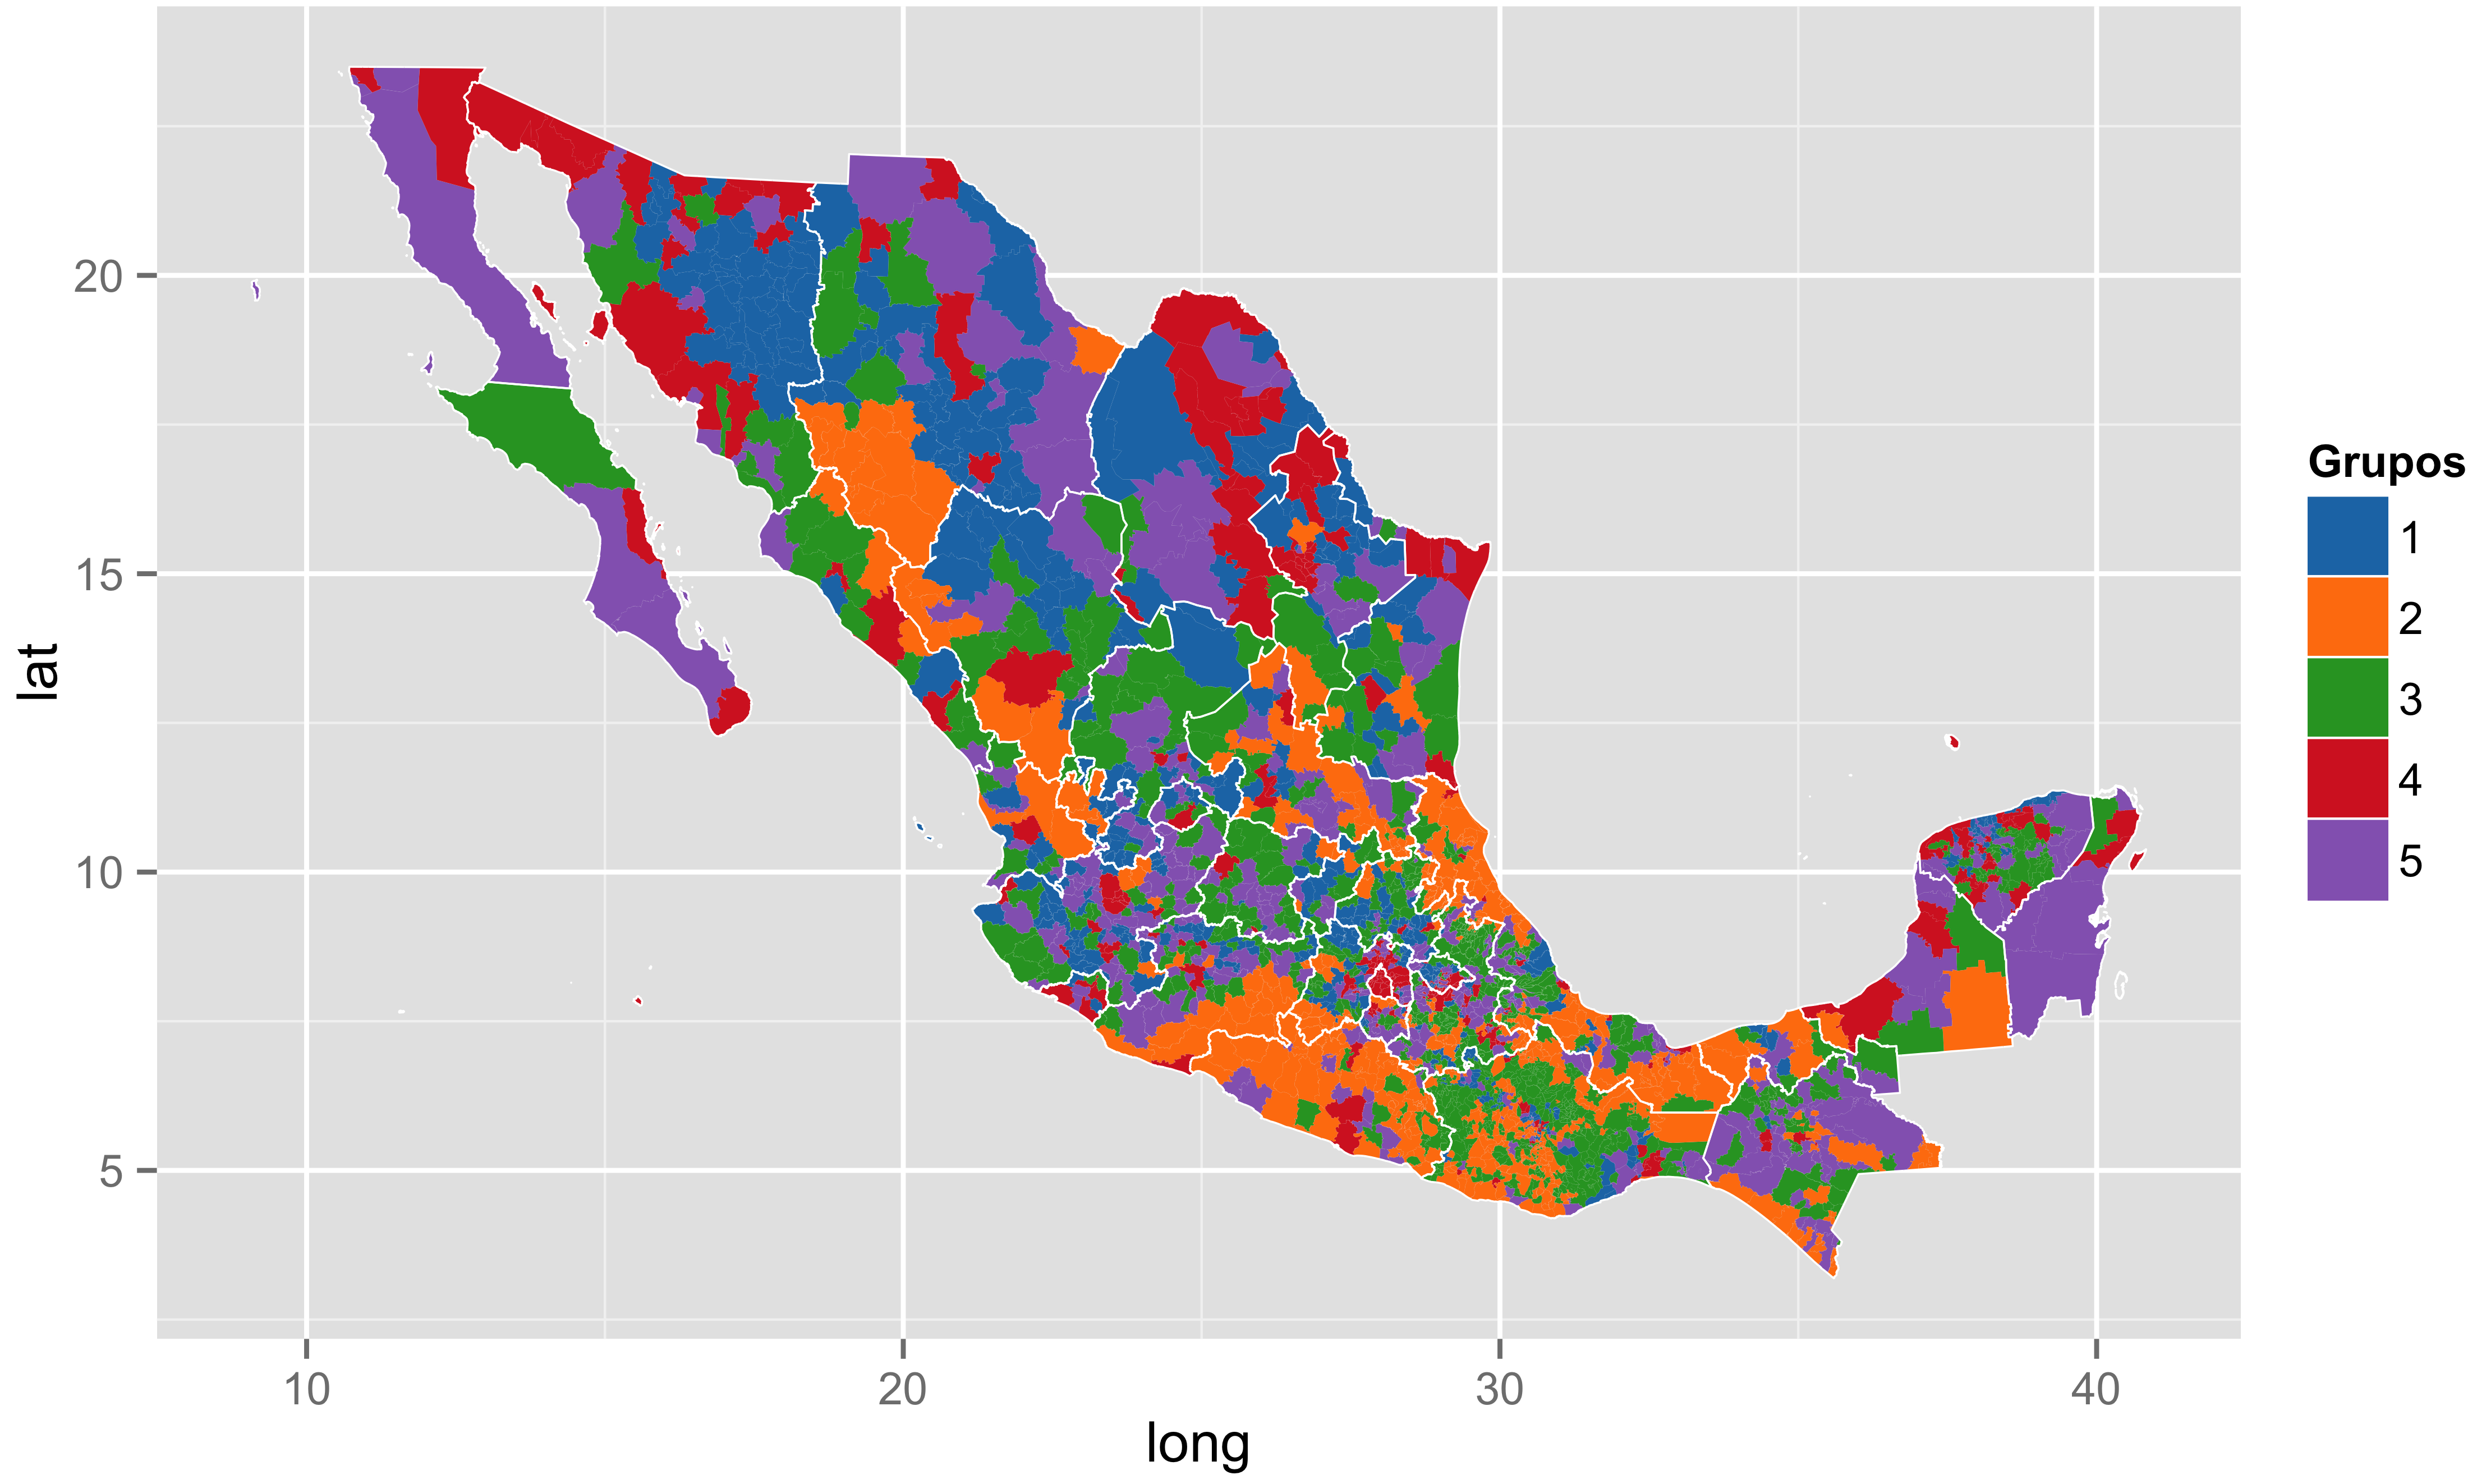
\includegraphics[width=\linewidth]{./maps/map5g.png}
    \caption{Obtenido}
  \endminipage\hfill
  \minipage{0.5\textwidth}
    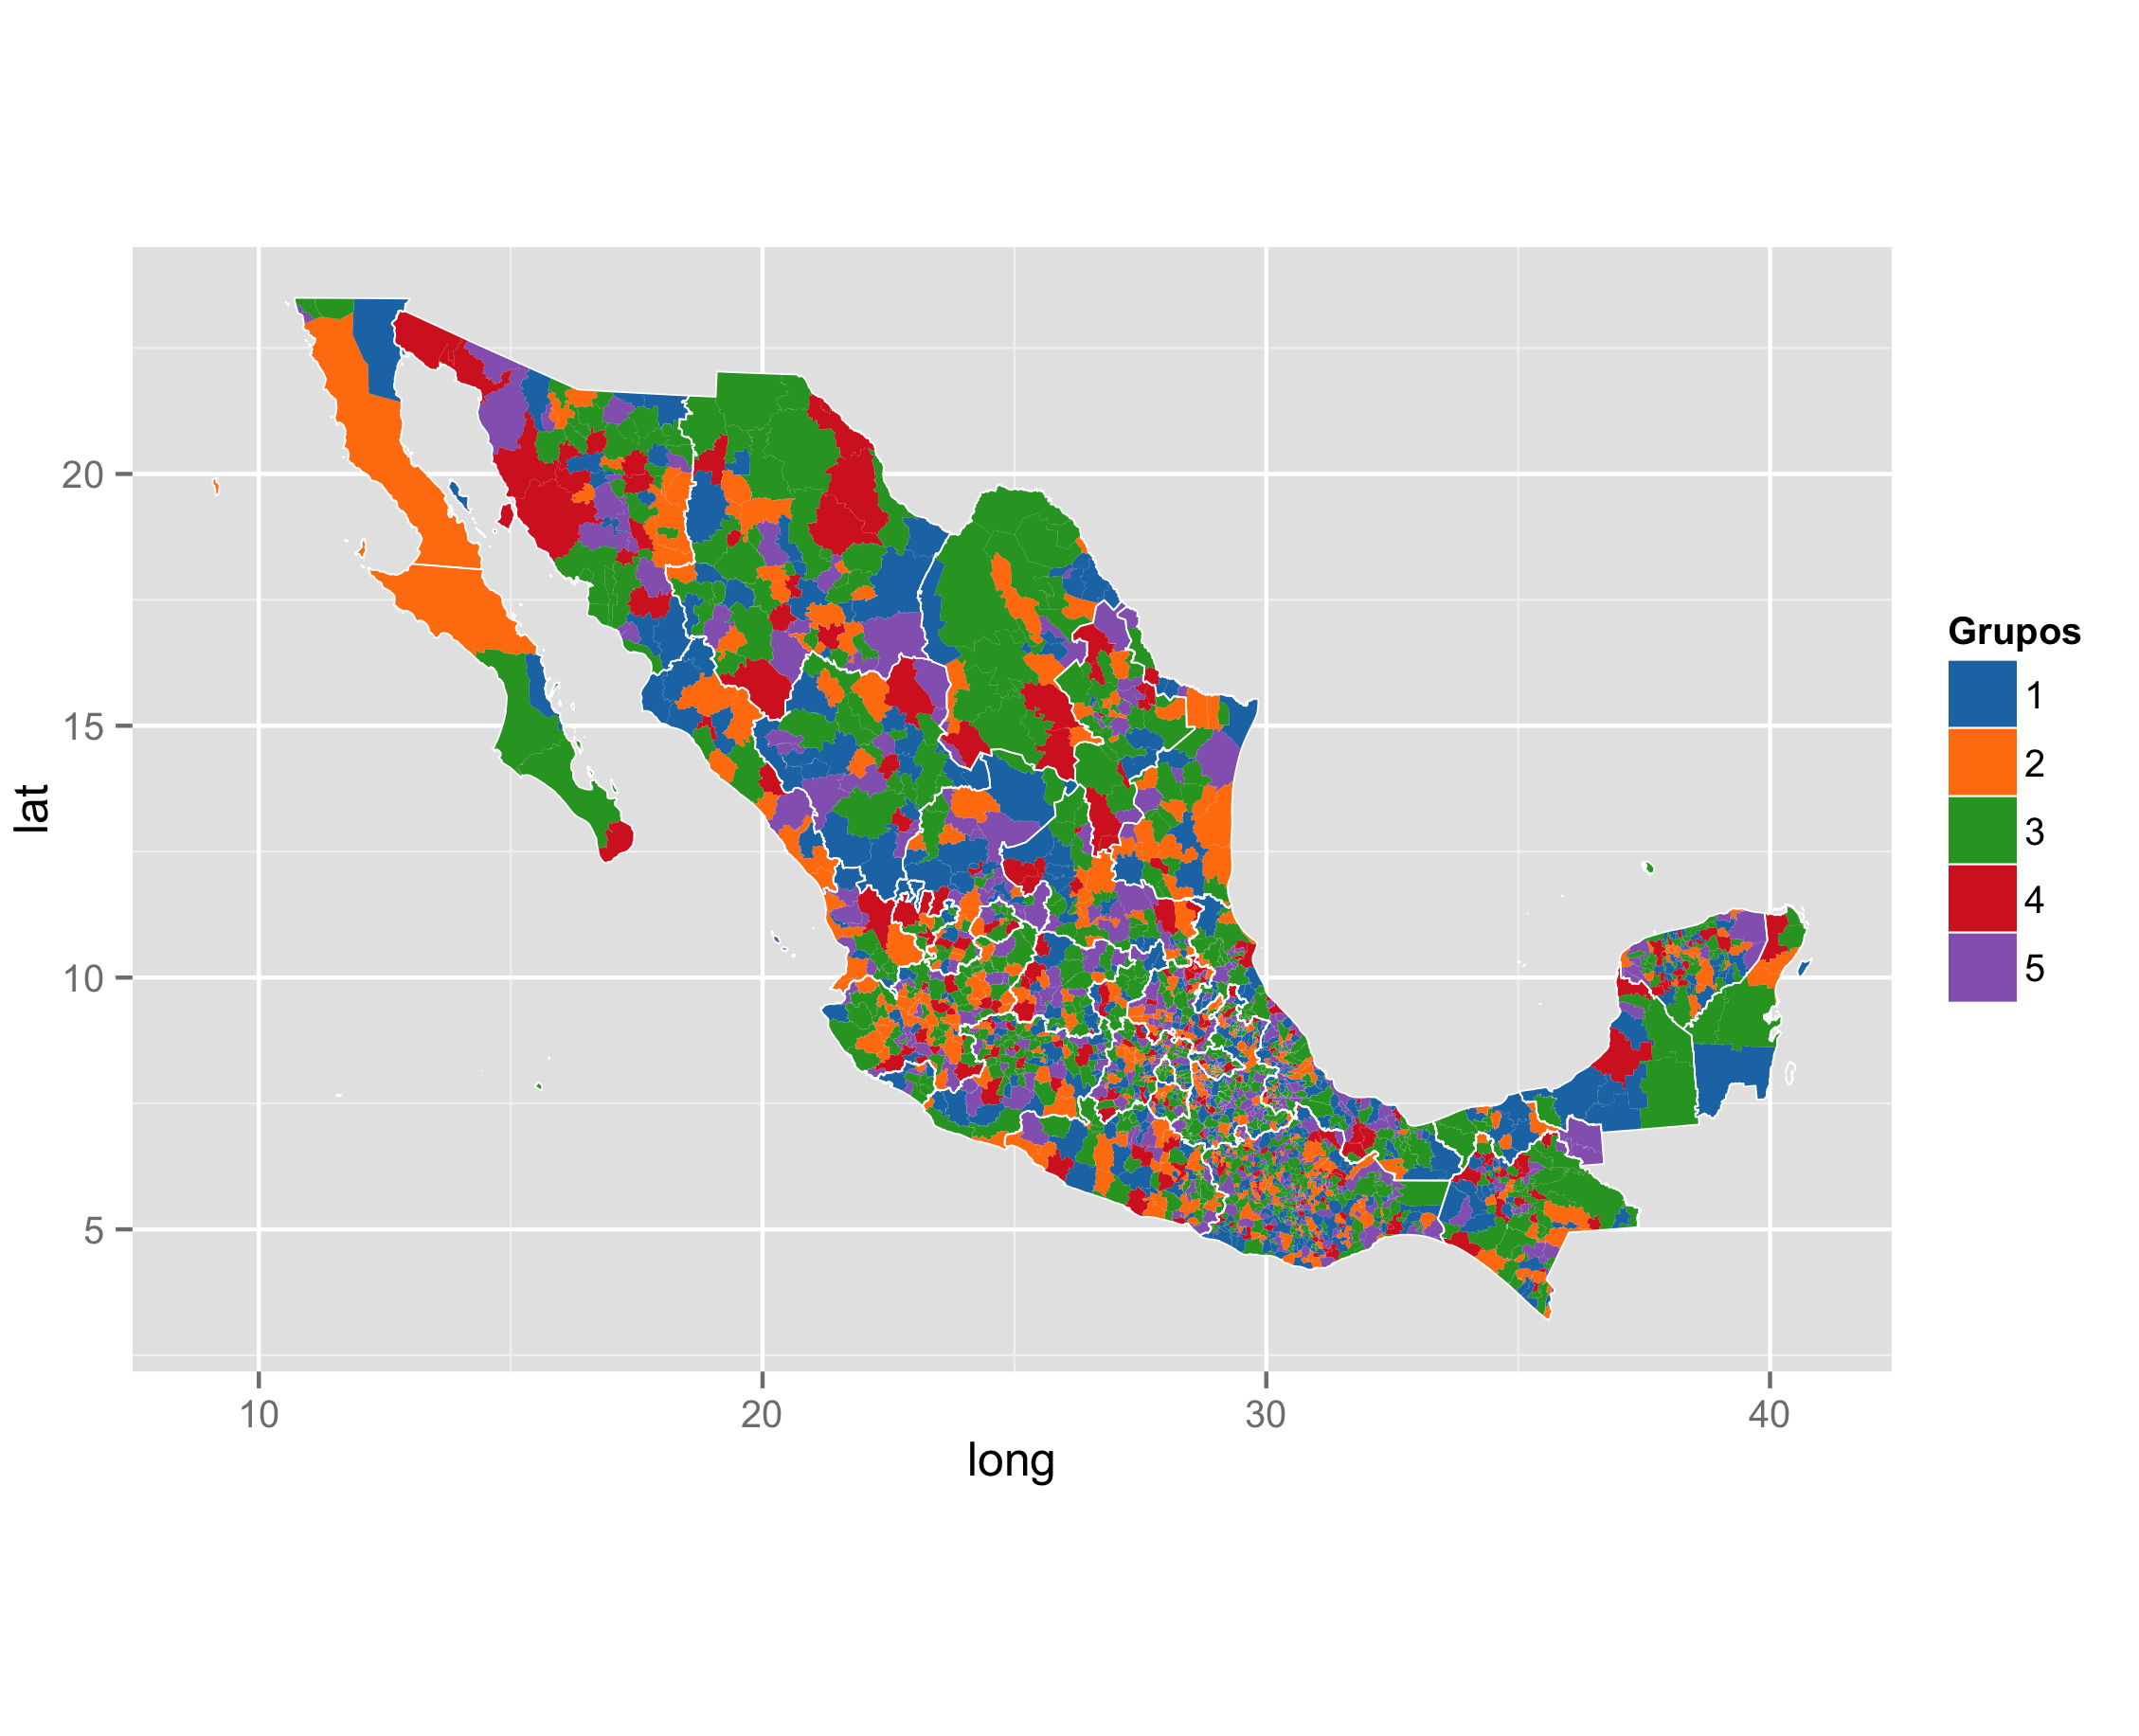
\includegraphics[width=\linewidth]{./maps/rmap5g.png}
    \caption{Aleatorizado}
  \endminipage\hfill
  \end{figure}
  A ojo parece que sí...
\end{frame}

\begin{frame}{Pruebas de Autocorrelación Espacial para los clusters}
  \begin{itemize}
    \item Uilizando el estadístico de conteo de fronteras del mismo color $N_{rr}$, con $r=1,2,\dots,5$, bajo muestreo sin reemplazo se obtiene:
    \item Bajo supuesto de normalidad:
    \begin{table}[ht]
      \centering
      \begin{tabular}{rrrrrr}
        \hline
        grupo & $\Hat{N_{rs}}$  & $N_{rs,0}$ & $\Var$ & $z$ & valor-p \\ 
        \hline
        1 & 98.61 & 48.80 & 6.53 & 19.49 & $< 2.2 \times 10^{-16}$ \\ 
        2 & 110.35 & 42.07 & 5.77  & 28.43 & $< 2.2 \times 10^{-16}$ \\ 
        3 & 194.99 & 132.80 & 14.00 & 16.62 & $< 2.2 \times 10^{-16}$ \\ 
        4 & 50.36 & 15.23 & 2.36 & 22.88 & $< 2.2 \times 10^{-16}$ \\ 
        5 & 63.59 & 37.40 & 5.22 & 11.46 & $< 2.2 \times 10^{-16}$ \\ 
         \hline
      \end{tabular}
    \end{table}
    \item En todos los casos rechazamos la hipótesis nula de no autocorrelación espacial.
  \end{itemize}

\end{frame}

\begin{frame}
Utilizando simulaciones de Monte Carlo con $n_{sim}=9999$:
  \begin{figure}[!ht]
    \centering
    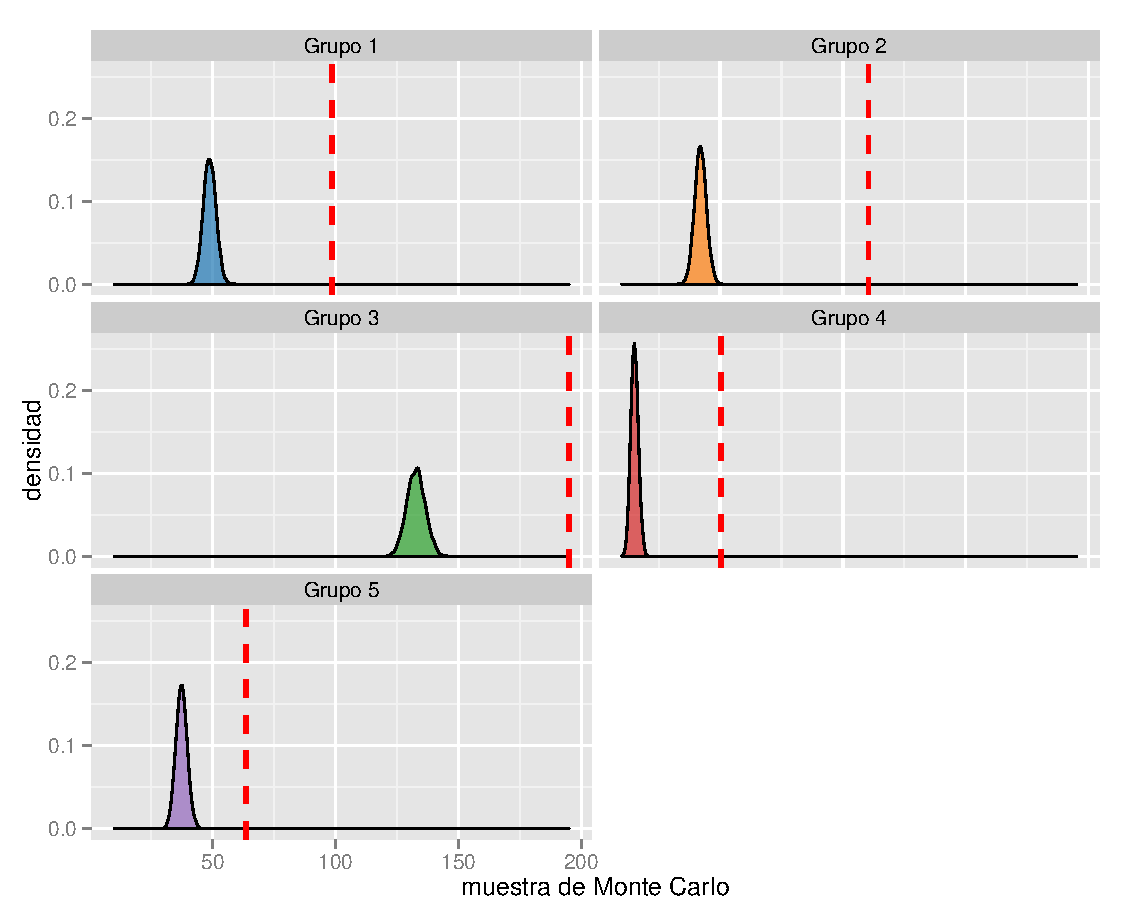
\includegraphics[width=.6\textwidth]{./plots/jc_density.pdf}
    \caption{Densidad de la muestra de Monte Carlo de $N_{rr}$. La línea punteada índica donde se encuentra $\Hat{N_{rr}}$. \label{obj:jcdensity} }
  \end{figure}
\end{frame}

\section{Conclusiones}
\begin{frame}{Conclusiones}
  \begin{itemize}
    \item Las pruebas sobre los índices $\mathcal{I}$ y $\mathcal{C}$ mostraron alta autocorrelación espacial positiva para el índice de marginación.

    \item Dentro del análisis de conglomerados, el estadístico Gap mostró que 5 es un número óptimo de grupos y se utilizó el algoritmo de $k$-medias esféricas para hacer los conglomerados. 

    \item Para comprobar la autocorrelación espacial positiva de los grupos obtenidos, se utilizaron los estadísticos $N_{ss}$ de conteo de fronteras. Los conteos entre fronteras del mismo grupo son significativamente mayores a los conteos esperados, indicando un grado de asociación espacial alto.

    \item A partir del análisis de conglomerados esférico, se encontró una estructura espacial latente para los datos de marginación.
  \end{itemize}
\end{frame}


\begin{frame}{Importancia del estudio}
  \begin{itemize}
    \item Este estudio nos permite identificar aglomeraciones en el mapa y conocer las necesidades de éstas. 
    \item Esto permite definir estrategias en materia de infraestructura para poder atender las carencias o necesidades de cada uno de los municipios. 
    \item Por ejemplo, la instalación de centros de salud o de atención en una zona céntrica en la Sierra Tarahumara. 

    \item Es importante señalar que la marginación de un municipio podría estar correlacionada con otras variables, como la dificultad de acceso o las condiciones geográficas del municipio.
  \end{itemize}
\end{frame}

\begin{frame}{Otros enfoques posibles}
  \begin{itemize}
    \item Podría realizarse un análisis similar para identificar focos rojos de violencia, necesidades en cuestión de salud e incluso para identificar segmentos de mercado por región.
    \item Si quisiéramos hacer un estudio más puntual, podríamos realizar el mismo estudio a nivel AGEB (Área Geoestadística Básica) o por manzana, enfocándonos en una región específica.
    \item También es posible realizar estudios espacio-temporales para ver la evolución de la marginación de los municipios a través del tiempo.
  \end{itemize}
\end{frame}

\begin{frame}
\centering
  \Huge{¡Muchas gracias!}
\end{frame}
% \begin{frame}{Blocks}
% \begin{block}{Block Title}
% You can also highlight sections of your presentation in a block, with it's own title
% \end{block}
% \begin{theorem}
% There are separate environments for theorems, examples, definitions and proofs.
% \end{theorem}
% \begin{example}
% Here is an example of an example block.
% \end{example}
% \end{frame}

% % Placing a * after \section means it will not show in the
% % outline or table of contents.
% \section*{Summary}

% \begin{frame}{Summary}
%   \begin{itemize}
%   \item
%     The \alert{first main message} of your talk in one or two lines.
%   \item
%     The \alert{second main message} of your talk in one or two lines.
%   \item
%     Perhaps a \alert{third message}, but not more than that.
%   \end{itemize}
  
%   \begin{itemize}
%   \item
%     Outlook
%     \begin{itemize}
%     \item
%       Something you haven't solved.
%     \item
%       Something else you haven't solved.
%     \end{itemize}
%   \end{itemize}
% \end{frame}



% % All of the following is optional and typically not needed. 
% \appendix
% \section<presentation>*{\appendixname}
% \subsection<presentation>*{For Further Reading}

% \begin{frame}[allowframebreaks]
%   \frametitle<presentation>{For Further Reading}
    
%   \begin{thebibliography}{10}
    
%   \beamertemplatebookbibitems
%   % Start with overview books.

%   \bibitem{Author1990}
%     A.~Author.
%     \newblock {\em Handbook of Everything}.
%     \newblock Some Press, 1990.
 
    
%   \beamertemplatearticlebibitems
%   % Followed by interesting articles. Keep the list short. 

%   \bibitem{Someone2000}
%     S.~Someone.
%     \newblock On this and that.
%     \newblock {\em Journal of This and That}, 2(1):50--100,
%     2000.
%   \end{thebibliography}
% \end{frame}

\end{document}


